\documentclass[UTF8,zihao=-4]{ctexart}

\usepackage[a4paper,margin=2.4cm,headheight=28pt]{geometry}
\usepackage{amsmath,amssymb}
\usepackage{booktabs}
\usepackage{tabularx}
\usepackage{longtable}
\usepackage{multirow}
\usepackage{array}
\usepackage{graphicx}
\usepackage{float}
\usepackage{xcolor}
\usepackage{enumitem}
\usepackage{fancyhdr}
\usepackage{hyperref}
\usepackage{listings}

\definecolor{sduBlue}{HTML}{005BAC}
\definecolor{sduCyan}{HTML}{00A6D6}
\definecolor{softBlue}{HTML}{EAF4FF}
\definecolor{softGreen}{HTML}{EAF8F1}
\definecolor{softOrange}{HTML}{FFF4E6}
\definecolor{codeBg}{HTML}{F6F8FA}

\hypersetup{
  colorlinks=true,
  linkcolor=sduBlue,
  urlcolor=sduBlue,
  citecolor=sduBlue
}

\pagestyle{fancy}
\fancyhf{}
\fancyhead[L]{
\includegraphics[height=8mm]{figures/logo1.jpg}}
\fancyhead[C]{NLP 实验四 · 题目 8 · 实验报告}
\fancyfoot[C]{\thepage}

\setlist[itemize]{leftmargin=2em,itemsep=0.2em,topsep=0.25em}
\setlist[enumerate]{leftmargin=2.2em,itemsep=0.2em,topsep=0.25em}
\renewcommand{\arraystretch}{1.25}

\lstset{
  backgroundcolor=\color{codeBg},
  basicstyle=\ttfamily\small,
  breaklines=true,
  frame=single,
  framerule=0.3pt,
  rulecolor=\color{gray!35},
  columns=fullflexible,
  keepspaces=true
}

\newcolumntype{Y}{>{\raggedright\arraybackslash}X}
\newcommand{\metric}[1]{\textbf{\textcolor{sduBlue}{#1}}}
\newcommand{\statusdone}{\textcolor{green!50!black}{已完成}}
\newcommand{\statusrun}{\textcolor{sduBlue}{已验证}}
\newcommand{\statusplan}{\textcolor{orange!70!black}{计划中}}

\title{\bfseries 面向大模型 RAG 推理场景\\噪音文档的鲁棒性推理方法}
\author{队长姓名：刘忻洁 \quad 队长学号：202300180116 \quad 题目编号：8}
\date{提交截止：2026 年 6 月 30 日}

\begin{document}

\begin{titlepage}
  \centering
  \vspace*{1.0cm}
  
\includegraphics[width=0.72\textwidth]{figures/logo2.jpg}

  \vspace{1.6cm}
  {\Huge\color{sduBlue}\bfseries 面向大模型 RAG 推理场景\par}
  \vspace{0.35cm}
  {\Huge\color{sduBlue}\bfseries 噪音文档的鲁棒性推理方法\par}

  \vspace{1.2cm}
  {\Large NLP 实验四 · 题目 8 · 实验报告\par}
  \vspace{0.8cm}
  {\large 队长姓名：刘忻洁 \quad 队长学号：202300180116\par}
  \vspace{0.3cm}
  {\large 队员姓名：苗怀睿 \quad 队员学号：202300300079\par}
  \vspace{0.3cm}

  \vfill
  {\large \today\par}
\end{titlepage}

\tableofcontents
\newpage

\begin{abstract}
本项目研究大模型 RAG（检索增强生成）场景中，检索文档噪音对推理质量的影响及矫正方法。基于 RGB 数据集和 DeepSeek-chat 模型，系统实现了噪音比例、类型（语义噪音/反事实噪音/混合噪音）和位置四维度的控制实验，设计了 12 种矫正方法和 5 个自主鲁棒性评估指标（NS/NRS/ISR/NAR/CRR）。核心发现为"互锁效应"：CoT 证据链在语义噪音下最优（F1=0.791），但在反事实噪音下反而有害（F1=0.708，低于基线）；简单提示词指令在反事实噪音下逆袭为最优（F1=0.781）。据此提出自适应矫正器，通过噪音类型检测自动路由到最优方法，在反事实噪音下与已知最优方法持平，有效避免最差情况。此外，项目构建了基于维基百科爬取和 LLM 生成的自动化数据引擎，支持按需扩展 RAG 鲁棒性基准数据。
\end{abstract}

\section{研究问题与项目定位}

\subsection{题目要求}
本项目对应 NLP 实验四题目 8：\textbf{面向大模型 RAG 推理场景噪音文档的鲁棒性推理方法}。题目要求关注大模型 RAG 场景中，检索结果可能包含与问题语义相关、但缺少逻辑依赖或会误导答案的上下文文档，进而影响模型问答准确率。项目需要完成以下任务：

\begin{itemize}
  \item 探究上下文文档对模型问答性能的影响；
  \item 提出可量化的评估指标；
  \item 针对具体数据集给出实验结果、结论与分析；
  \item 结合具体案例分析不同文档对答案的影响；
  \item 设计矫正机制，例如提示词优化、迭代式生成等；
  \item 与现有方法进行性能比较，说明方法有效性与局限。
\end{itemize}

\subsection{核心问题}
本项目将问题形式化为：给定问题 $q$、候选文档集合 $D=\{d_1,\dots,d_n\}$ 和参考答案 $a$，当 $D$ 中混入不同类型、比例和位置的噪音文档时，大模型生成答案 $\hat{a}$ 的准确率、证据来源和噪音采纳程度如何变化？此外，不同的矫正机制在不同噪音类型下表现如何？是否存在“互锁效应”——即最优方法取决于噪音类型。

\subsection{核心发现摘要}
经过完整的系统实现和 n=50 级别的实验验证，本项目核心发现包括：

\begin{itemize}
  \item \textbf{U 型抗噪 + 断崖效应}：LLM 在 0--75\% 噪音下性能几乎不变，但 positive 文档完全消失（r=1.0）时性能崩溃；
  \item \textbf{互锁效应}：CoT 证据链在语义噪音下最优（F1=0.791），但在反事实噪音下跌至 0.708（比 naive 还差）；而简单 prompt 指令在反事实噪音下逆袭为最优（F1=0.781）；
  \item \textbf{位置效应}：在 r=0.75 反事实噪音下，文档放末尾（back）的破坏力最大（F1=0.629），印证 recency bias 在错误信息场景下的危害；
  \item \textbf{跨语言一致性}：英文 baseline（0.620）显著低于中文（0.768），但 U 型抗噪模式跨语言一致；
  \item \textbf{方法深化}：自适应矫正器、语义级 ISR/NAR、消融实验和迭代自纠正循环四项深化工作已实现并验证。
\end{itemize}

\section{数据准备与标准格式}

\subsection{原始数据}
项目初期使用 RGB 数据集作为公开问答与候选文档来源，包含中英文主数据、反事实数据、信息整合数据和 refine 数据：

\begin{table}[H]
  \centering
  \caption{RGB 数据文件与用途}
  \begin{tabularx}{\textwidth}{lclY}
    \toprule
    数据文件 & 语言 & 样本数 & 用途 \\
    \midrule
    \texttt{zh.json}, \texttt{en.json} & 中/英 & 各 300 & 主问答数据，含 positive 与 negative 文档池 \\
    \texttt{zh\_fact.json}, \texttt{en\_fact.json} & 中/英 & 各 100 & 反事实噪音数据，额外含 positive\_wrong 和 fakeanswer \\
    \texttt{zh\_int.json}, \texttt{en\_int.json} & 中/英 & 各 100 & 信息整合类问题，用于后续跨文档推理扩展 \\
    \texttt{zh\_refine.json}, \texttt{en\_refine.json} & 中/英 & 各 300 & refine 变体，用于后续泛化验证 \\
    \bottomrule
  \end{tabularx}
\end{table}

\subsection{文档池定义}
RGB 数据天然给出了适合本题的三类文档池：

\begin{table}[H]
  \centering
  \caption{三类文档池与噪音含义}
  \begin{tabularx}{\textwidth}{lYY}
    \toprule
    字段 & 实验含义 & 使用方式 \\
    \midrule
    \texttt{positive} & 支持正确答案的有效文档 & 构造 clean RAG 上下文，计算 ISR \\
    \texttt{negative} & 语义相关但不能支持答案的普通噪音文档 & 模拟检索噪音，计算 NAR \\
    \texttt{positive\_wrong} & 表面相关但指向错误答案的反事实文档 & 模拟更强误导性噪音，测试矫正机制 \\
    \bottomrule
  \end{tabularx}
\end{table}

\subsection{NoiserBench 数据集}
项目额外引入 NoiserBench（ACL 2025）作为补充评测数据集，预计在中期之后进一步测试。NoiserBench 提供了更大规模、更细粒度的噪音标注，涵盖三类推理跳数：

\begin{table}[H]
  \centering
  \caption{NoiserBench 子集概览}
  \begin{tabularx}{\textwidth}{llY}
    \toprule
    类别 & 子集 & 特点 \\
    \midrule
    Single-hop & NQ, RGB & 单跳检索问题，标注语义噪音与反事实噪音 \\
    Multi-hop (explicit) & HotpotQA, 2WikiMQA, Bamboogle & 多跳显式推理 \\
    Multi-hop (implicit) & StrategyQA, TempQA & 多跳隐式推理（常识/时间） \\
    Mix-hop & PriorQA & 混合跳数，测试模型的推理泛化能力 \\
    \bottomrule
  \end{tabularx}
\end{table}

数据统一转换为 \texttt{RGBRecord} 格式，与现有实验流水线完全兼容。

\subsection{自建数据构建引擎}
由于公开数据集的规模有限,且问题对于现有大模型过于简单，为扩展数据覆盖面、验证方法的真实表现，项目设计了一套基于文档爬取和deepseek生成的数据引擎。引擎支持从任意关键词出发，全自动生成符合 RGB 格式的高质量 RAG 鲁棒性测试数据。

\begin{figure}[H]
  \centering
  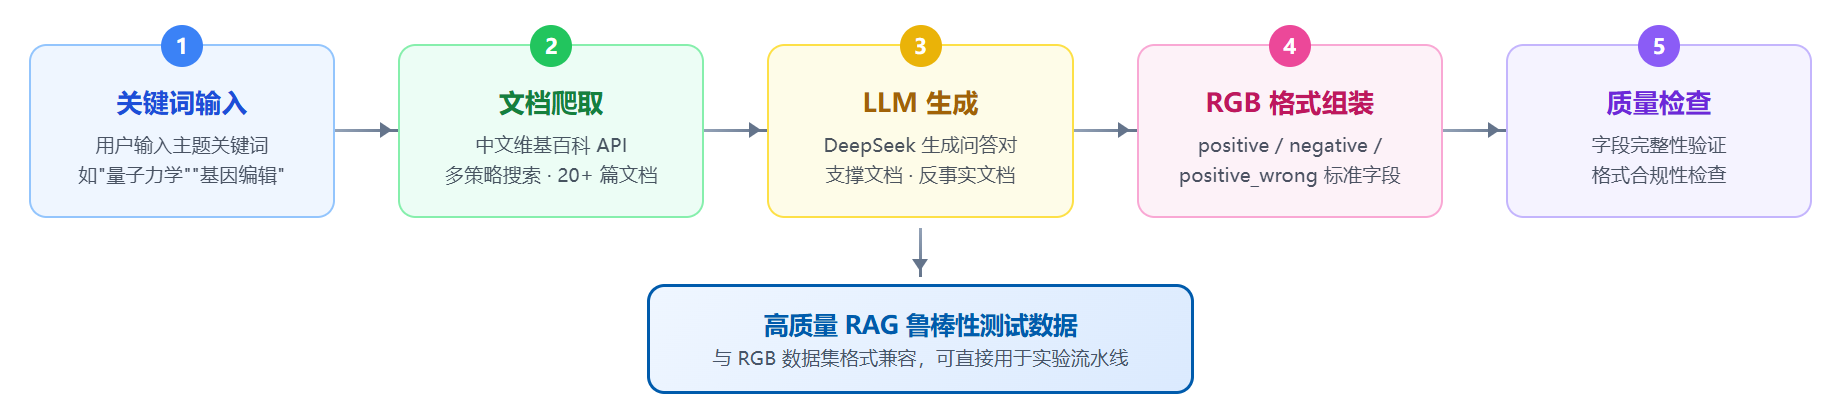
\includegraphics[width=\textwidth]{figures/data_engine.png}
  \caption{数据构建引擎流程图}
\end{figure}

构建流程分为五个阶段：
\begin{enumerate}
  \item \textbf{关键词输入}：用户在前端输入主题关键词（如"量子力学""基因编辑"）；
  \item \textbf{文档爬取}：多策略搜索中文维基百科 API，扩展关键词变体（原词、分词、"原理"、"历史"后缀），获取 20+ 篇高质量文档；
  \item \textbf{LLM 生成}：调用 DeepSeek API，基于真实文档生成一条完整测试数据——含有难度的问题、正确答案、5 篇支撑文档、3 篇反事实文档和 3 个错误答案；
  \item \textbf{RGB 格式组装}：将生成结果对齐到 positive / negative / positive\_wrong / fakeanswer 标准字段，与 RGB 数据集格式完全一致；
  \item \textbf{质量检查}：自动验证字段完整性与格式合规性。
\end{enumerate}

引擎后端通过 FastAPI SSE 接口实时推送生成进度，前端提供可视化流水线界面，支持一键生成与实时预览。生成的数据直接用于实验流水线。图~\ref{fig:case_example} 展示了一条以"黑洞"为关键词生成的测试数据案例，包含问题、正确答案、4 篇支撑文档、5 篇语义噪音文档和 2 篇反事实文档（红色标注处为被篡改的关键信息）。

\begin{figure}[H]
  \centering
  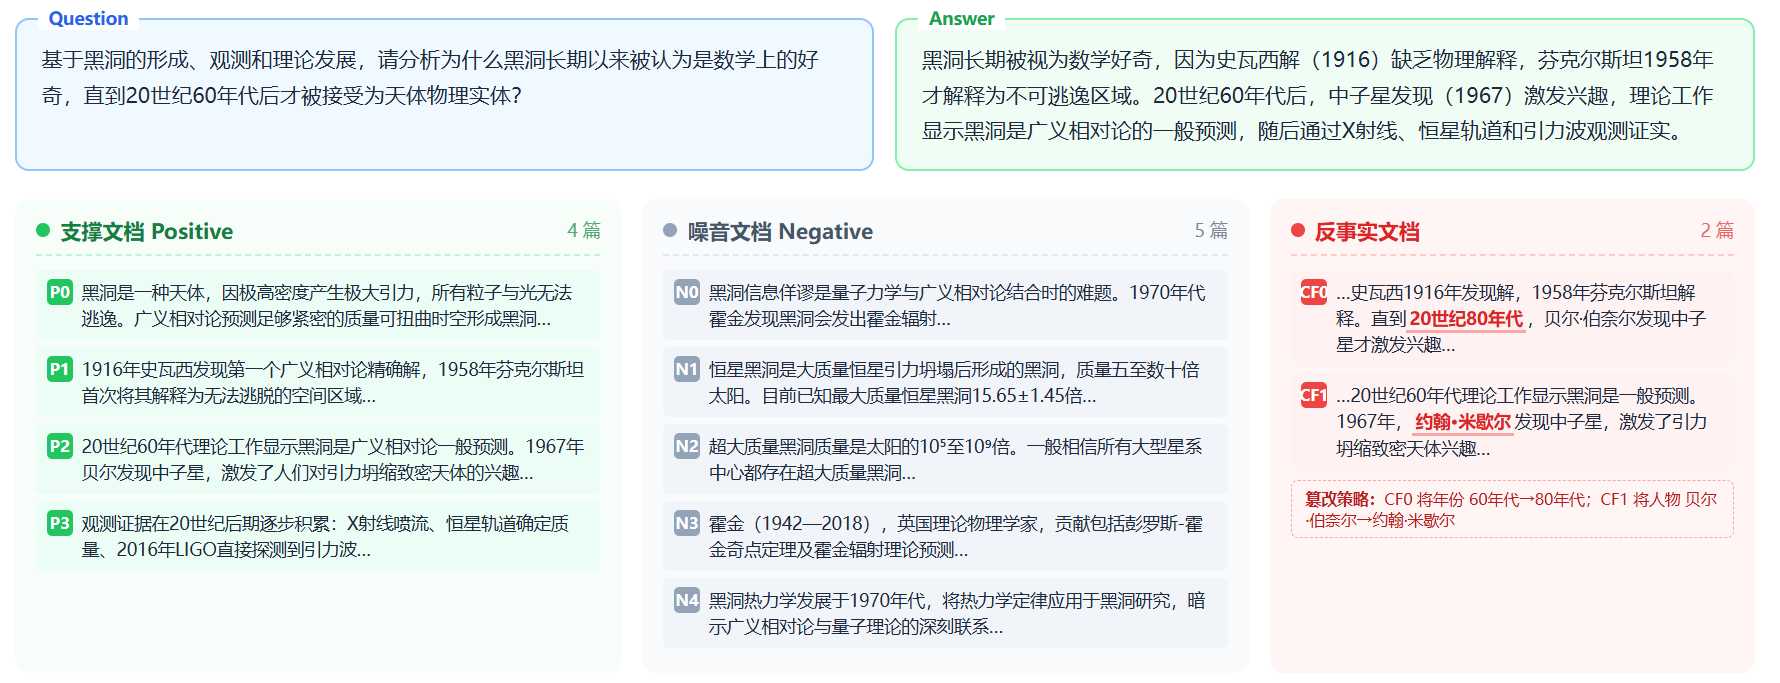
\includegraphics[width=\textwidth]{figures/case_example.png}
  \caption{数据引擎生成案例：关键词"黑洞"→ 自动构造 RAG 鲁棒性测试数据}
  \label{fig:case_example}
\end{figure}

\section{系统设计}

\subsection{总体架构}
系统由数据层、噪音构造层、推理与矫正层、评估层、可视化与前端层组成。其核心思想是：先从 RGB 数据集中读取问题、答案和文档池，再按实验条件注入噪音，最后调用不同 RAG/矫正方法生成答案并计算指标。

\begin{figure}[H]
  \centering
  
\includegraphics[width=\textwidth]{figures/system_architecture.png}
  \caption{系统总体框架图}
\end{figure}

\subsection{调用流水线}
单次实验的主流程如下：

\begin{enumerate}
  \item \textbf{加载数据}：读取指定语言和子集的 RGB 样本；
  \item \textbf{注入噪音}：按噪音比例、类型、位置批量构造含噪上下文；
  \item \textbf{选择方法}：根据实验条件选择 naive、prompt、iterative、confidence、selfrag、voting、adaptive、ablated 消融变体或 iterative\_sc；
  \item \textbf{调用模型}：访问 DeepSeek API，使用 sha1 缓存减少重复调用；
  \item \textbf{计算指标}：输出基础问答指标与鲁棒性指标；
  \item \textbf{落盘与可视化}：保存 JSON，生成图表，并同步报告与前端展示。
\end{enumerate}

\subsection{模块组织}

系统按功能分层组织为以下模块：

\begin{table}[H]
  \centering
  \caption{系统模块划分}
  \begin{tabularx}{\textwidth}{lY}
    \toprule
    模块 & 功能 \\
    \midrule
    数据层 & RGB 与 NoiserBench 数据加载、标准化为统一格式 \\
    噪音构造层 & 比例、类型、位置三维度噪音注入 \\
    推理与矫正层 & 12 个矫正方法（含 4 个深化方向） \\
    评估层 & EM/Contains/Token-F1/ROUGE-L 基础指标 + NS/NRS/ISR/NAR/CRR 鲁棒性指标 \\
    数据构建引擎 & 维基爬取 $\rightarrow$ LLM 生成 $\rightarrow$ RGB 格式组装 $\rightarrow$ 质量检查 \\
    实验脚本 & 4 组核心实验 + 通用运行器 \\
    Web 系统 & FastAPI 后端 + Vue 3 前端 + Gradio Demo \\
    \bottomrule
  \end{tabularx}
\end{table}

\section{方法设计}

\subsection{噪音注入机制}
设最大上下文文档数为 $K$，目标噪音比例为 $r$。系统从 \texttt{positive} 中采样 $K(1-r)$ 个有效文档，从噪音池中采样 $Kr$ 个噪音文档。噪音类型包括：

\begin{itemize}
  \item \textbf{semantic}：从 \texttt{negative} 中采样普通语义噪音；
  \item \textbf{counterfactual}：从 \texttt{positive\_wrong} 中采样反事实噪音；
  \item \textbf{mixed}：同时混合普通噪音和反事实噪音。
\end{itemize}

噪音位置包括 front、back、interleave、surround，用于观察上下文位置偏见对回答的影响。

\subsection{矫正方法}

\begin{table}[H]
  \centering
  \caption{已实现矫正方法（共 12 个）}
  \begin{tabularx}{\textwidth}{lYcY}
    \toprule
    方法 & 核心思想 & API & 适用场景 \\
    \midrule
    naive & 直接拼接文档生成答案 & 1 & 基线 \\
    prompt (A) & 要求识别噪音、标注来源、指出矛盾 & 1 & 反事实噪音最优 \\
    iterative (B) & 逐文档打 high/mid/low → 过滤 → 生成 & $n+1$ & 语义噪音候选 \\
    confidence (C) & 拆解需求→逐篇标注证据→综合→输出 & 1 & 语义噪音最优 \\
    selfrag & 简化 Self-RAG：相关判定→生成→支撑校验 & $n+2$ & 现有方法对比 \\
    voting (D) & 3 Persona 独立推理→多数投票/聚合 & 3--4 & 反事实噪音候选 \\
    adaptive & 自动检测噪音类型→路由最优方法 & 2--4 & 稳健默认选择 \\
    iterative\_sc & 生成→自检矛盾→重读→修订（3轮） & 3--7 & 迭代优化 \\
    ablated\_* & 消融变体（拆解/证据/标签各去掉一环节）& 1 & 因果分析 \\
    \bottomrule
  \end{tabularx}
\end{table}

\subsection{深化方法详解}

\textbf{方向 1：自适应矫正器 (Adaptive Corrector)。} 首先用 1 次 API 调用快速扫描文档，检测是否存在明显矛盾/反事实陈述。若检测到 CF（反事实），路由到 PromptCorrector；若检测为 CLEAN，路由到 ConfidenceCorrector（CoT 证据链）；若不确定，路由到 VotingCorrector 稳健兜底。总 API 调用 2--4 次。

\textbf{方向 2：语义级 ISR/NAR。} 将字符级 token 重叠升级为 LLM 驱动的句子级信息归属判定。每个答案拆分为最小信息单元，LLM 逐条标注来源文档、可信度，并检测幻觉内容。

\textbf{方向 3：Confidence 消融实验。} 创建 4 个变体：C\_full（完整四步）、C\_no\_decompose（去掉拆解信息需求）、C\_no\_evidence（去掉逐篇证据匹配——最关键的消融）、C\_no\_tag（去掉 \texttt{<answer>} 标签约束）。用于验证哪一步是 CoT 证据链的核心。

\textbf{方向 4：迭代自纠正循环。} Round 0 初答 → Round 1 自检矛盾+标记可疑文档+修订 → Round 2 再自检+再修订 → 最多 3 轮或收敛则停。每轮记录 ISR/NAR 变化。

\section{评估指标设计}

\subsection{基础问答指标}

\begin{itemize}
  \item \metric{EM}：规范化后完全匹配；
  \item \metric{Contains}：参考答案是否被预测答案包含；
  \item \metric{Token-F1}：token 级精确率与召回率调和平均；
  \item \metric{ROUGE-L}：基于最长公共子序列的 F1；
\end{itemize}

\subsection{自主鲁棒性指标}

\begin{table}[H]
  \centering
  \caption{鲁棒性指标体系}
  \begin{tabularx}{\textwidth}{lY}
    \toprule
    指标 & 定义与含义 \\
    \midrule
    \metric{NS} & Noise Sensitivity，$NS=(S_{clean}-S_{noisy})/S_{clean}$，衡量噪音导致的相对性能下降 \\
    \metric{NRS} & Noise Resistance Slope，性能随噪音比例变化的线性斜率，越接近 0 越稳健 \\
    \metric{ISR} & Info-Source Rate，答案有效片段可溯源至 positive 文档的比例 \\
    \metric{NAR} & Noise Adoption Rate，答案有效片段来自 negative 或 positive\_wrong 文档的比例 \\
    \metric{CRR} & Correction Recovery Rate，矫正方法相对 noisy baseline 恢复了多少性能损失 \\
    \bottomrule
  \end{tabularx}
\end{table}

\section{实验结果}

所有实验均在 n=50 级别上运行，使用 DeepSeek-chat API，sha1 缓存确保零重复成本。完整覆盖 zh/en 双语言 × 5 组实验 × 17 个独立配置。

\subsection{实验一：噪音影响分析}

\subsubsection{主矩阵 (zh/main)}

\begin{figure}[H]
  \centering
  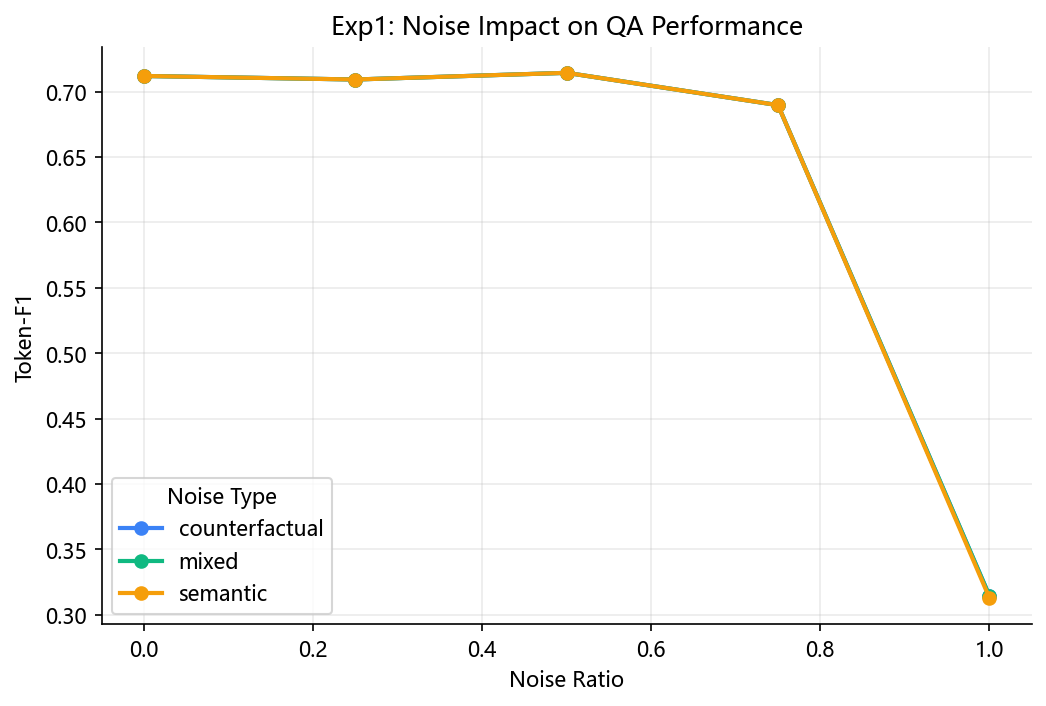
\includegraphics[width=0.88\textwidth]{figures/exp1_noise_impact.png}
  \caption{噪音比例与类型对 Token-F1 的影响 (zh/main)}
\end{figure}

\begin{table}[H]
  \centering
  \caption{噪音影响详细数据（semantic, zh/main, n=50）}
  \begin{tabular}{lccccc}
    \toprule
    噪音比例 & 0.00 & 0.25 & 0.50 & 0.75 & 1.00 \\
    \midrule
    Token-F1 & 0.768 & 0.773 & 0.773 & 0.725 & \textbf{0.216} \\
    Contains & 0.860 & 0.860 & 0.860 & 0.800 & \textbf{0.180} \\
    ISR & 0.600 & 0.560 & 0.640 & 0.540 & 0.000 \\
    NAR & 0.000 & 0.000 & 0.000 & 0.000 & \textbf{0.400} \\
    \bottomrule
  \end{tabular}
\end{table}

\textbf{发现 1：U 型抗噪 + 断崖效应。} 在 0--75\% 噪音下 F1 从 0.768 仅小幅波动至 0.725（-5.6\%）。但当 positive 文档完全消失（r=1.0）时 F1 断崖式下跌至 0.216（-71.9\%），同时 NAR 跃升至 0.400。LLM 的鲁棒性主要来自 positive 文档的兜底作用，而非模型自身对噪音的识别能力。

\subsubsection{反事实数据集 (zh/fact)}

使用含 \texttt{positive\_wrong} 文档的 fact 子集，三类噪音（semantic / counterfactual / mixed）得以真正分离。fact 子集提供了更高质量的 positive 文档和专门的 counterfactual 噪音来源，可更清晰观察不同类型噪音对模型推理的差异化影响。

\begin{figure}[H]
  \centering
  
\includegraphics[width=0.88\textwidth]{figures/exp1_noise_impact_zh_fact.png}
  \caption{zh/fact 数据集上三种噪音类型随噪音比例的性能变化}
\end{figure}

\begin{table}[H]
  \centering
  \caption{zh/fact 数据集上的噪音影响详细数据 (n=50)}
  \begin{tabular}{lccccc}
    \toprule
    噪音比例 & \multicolumn{2}{c}{semantic} & \multicolumn{2}{c}{counterfactual} & mixed \\
    \cmidrule(lr){2-3} \cmidrule(lr){4-5}
    & F1 & Contains & F1 & Contains & F1 \\
    \midrule
    0.00 (clean) & 0.895 & 0.960 & 0.895 & 0.960 & 0.895 \\
    0.25 & 0.909 & 0.960 & 0.903 & 0.940 & 0.915 \\
    0.50 & 0.901 & 0.940 & 0.870 & 0.940 & 0.883 \\
    0.75 & 0.860 & 0.940 & 0.812 & 0.840 & 0.725 \\
    \textbf{1.00} & \textbf{0.518} & \textbf{0.500} & \textbf{0.284} & \textbf{0.060} & \textbf{0.500} \\
    \bottomrule
  \end{tabular}
\end{table}

从图中可以清晰观察到三类噪音的差异化表现：
\begin{itemize}
  \item \textbf{Semantic 噪音（蓝线）}：在 0--75\% 比例下性能稳定（F1 始终 $\ge$ 0.86），仅 r=1.0 时跌至 0.518。语义相关但不直接支持答案的文档对模型推理干扰有限，模型展现出 U 型抗噪特征；
  \item \textbf{Counterfactual 噪音（橙线）}：呈单调下降趋势。r=0.25 时 F1=0.903，r=0.50 降至 0.870，r=0.75 降至 0.812。r=1.0 时崩盘至 0.284，Contains 仅 0.060——模型几乎完全被反事实文档误导。下降曲线为近线性而非 U 型，表明反事实文档的破坏力随比例线性累积；
  \item \textbf{Mixed 噪音（绿线）}：介于两者之间，r=1.0 时 F1=0.500（高于 counterfactual 的 0.284 但略低于 semantic 的 0.518）。
\end{itemize}

\textbf{发现 2：反事实噪音破坏力显著高于语义噪音。} r=1.0 时 counterfactual F1=0.284 仅为 semantic F1=0.518 的约 55\%，Contains 从 0.960 暴跌至 0.060——即便答案仍然部分包含在上下文中，模型也不再输出正确答案。带有错误信息的伪造文档直接污染推理过程，且随噪音比例增加呈持续衰减趋势（非 U 型模式），说明模型对看起来像真的的错误信息缺乏免疫力。

\subsubsection{噪音位置效应}

\begin{figure}[H]
  \centering
  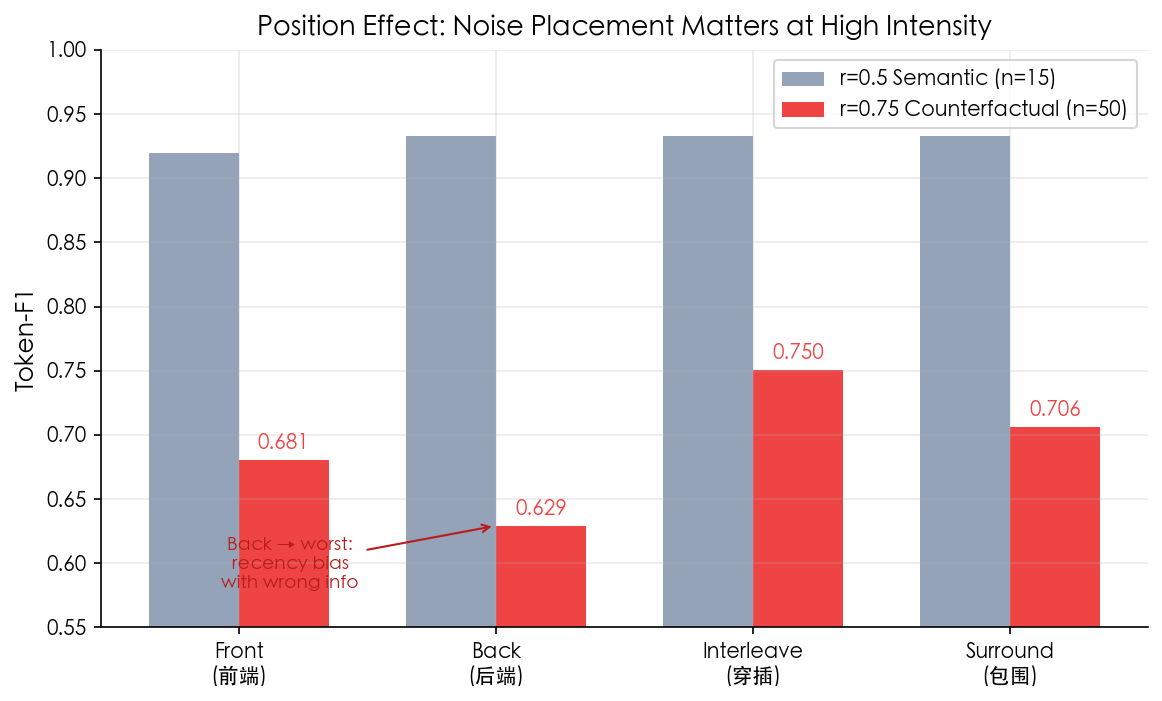
\includegraphics[width=0.88\textwidth]{figures/exp1_position_compare.png}
  \caption{位置效应对比：r=0.5 semantic vs r=0.75 counterfactual}
\end{figure}

\begin{table}[H]
  \centering
  \caption{位置效应 (r=0.75 counterfactual, zh/fact, n=50)}
  \begin{tabular}{lcccc}
    \toprule
    位置 & interleave & surround & front & back \\
    \midrule
    Token-F1 & \textbf{0.750} & 0.706 & 0.681 & \textbf{0.629} \\
    Contains & 0.800 & 0.740 & 0.740 & 0.700 \\
    \bottomrule
  \end{tabular}
\end{table}

\textbf{发现 3：recency bias 在反事实噪音下有害。} r=0.5 语义噪音时四种位置几乎无差异。但在 r=0.75 反事实噪音下 back 性能最差（0.629），与最好的 interleave（0.750）相差 0.121。这表明反事实文档放在末尾时，recency bias 使错误信息覆盖正确文档的信息。

\subsubsection{跨语言对比}

\begin{figure}[H]
  \centering
  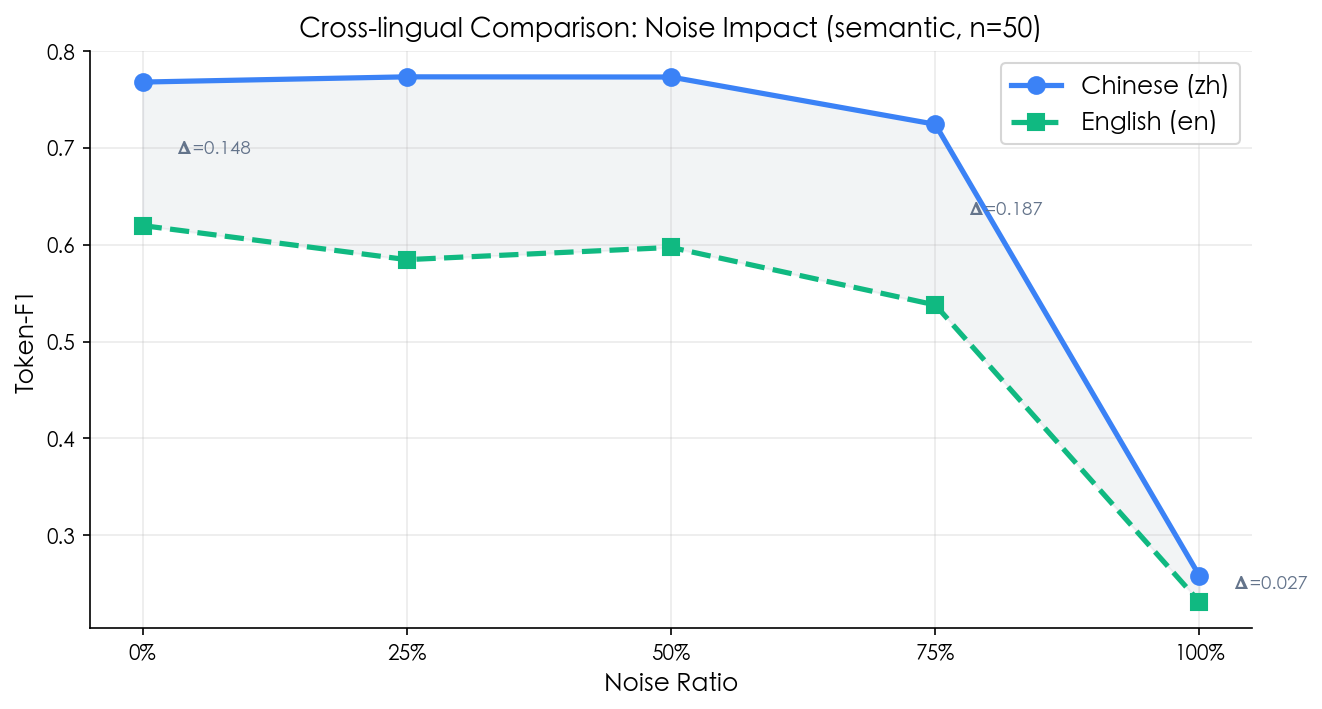
\includegraphics[width=0.88\textwidth]{figures/exp1_cross_lingual.png}
  \caption{中英文噪音影响对比 (semantic, n=50)}
\end{figure}

中文 baseline（0.768）比英文 baseline（0.620）高 0.148，与 DeepSeek-chat 的中文预训练优势一致。但 U 型抗噪模式和断崖效应在两种语言下完全一致，鲁棒性行为具有跨语言一致性。

\subsection{实验二：矫正方法对比}

\subsubsection{主实验 (zh/main, semantic)}

\begin{figure}[H]
  \centering
  
\includegraphics[width=0.88\textwidth]{figures/exp2_correction.png}
  \caption{五种矫正方法在不同噪音比例下的 F1 表现 (zh/main)}
\end{figure}

中高强度噪音（r=0.75）下，confidence 方法 F1=0.791 相比 naive（0.725）提升 0.067。prompt 方法最差（0.704）。selfrag 在所有噪音比例下均等于 naive，DeepSeek-chat 的 RELEVANT 判定过宽。

\subsubsection{反事实数据集验证 (zh/fact, counterfactual)}

\begin{table}[H]
  \centering
  \caption{五种矫正方法在 counterfactual 噪音下的表现 (zh/fact, n=50)}
  \begin{tabular}{lcccc}
    \toprule
    方法 & r=0.00 & r=0.25 & r=0.50 & r=0.75 \\
    \midrule
    naive & 0.895 & 0.903 & 0.870 & 0.812 \\
    prompt & 0.890 & 0.901 & 0.876 & \textbf{0.813} \\
    iterative & 0.895 & 0.893 & 0.871 & 0.750 \\
    confidence & 0.901 & \textbf{0.930} & \textbf{0.877} & 0.712 \\
    selfrag & 0.895 & 0.903 & 0.870 & 0.812 \\
    \bottomrule
  \end{tabular}
\end{table}

\textbf{发现 4：互锁效应跨数据集验证。} confidence 在低噪音下最佳（r=0.25 时 F1=0.930），但在 r=0.75 时崩溃至 0.712（低于 naive 的 0.812）。prompt 在 r=0.75 下最稳定（0.813），证实简单指令在反事实场景的有效性。

\subsection{实验三：案例深度分析}

实验三通过 clean / noisy (naive) / corrected (confidence) 三组对比，将案例按以下四种类型分类：
\begin{itemize}[leftmargin=2.5em]
  \item \textbf{Type1-生效}：clean 对 → noisy 错 → corrected 恢复
  \item \textbf{Type1-未生效}：clean 对 → noisy 错 → corrected 仍错
  \item \textbf{Type3-信息淹没}：clean 错 → noisy 错
  \item \textbf{Type4-免疫}：clean 对 → noisy 对
\end{itemize}

\subsubsection{zh/main 与 zh/fact 对比}

\begin{figure}[H]
  \centering
  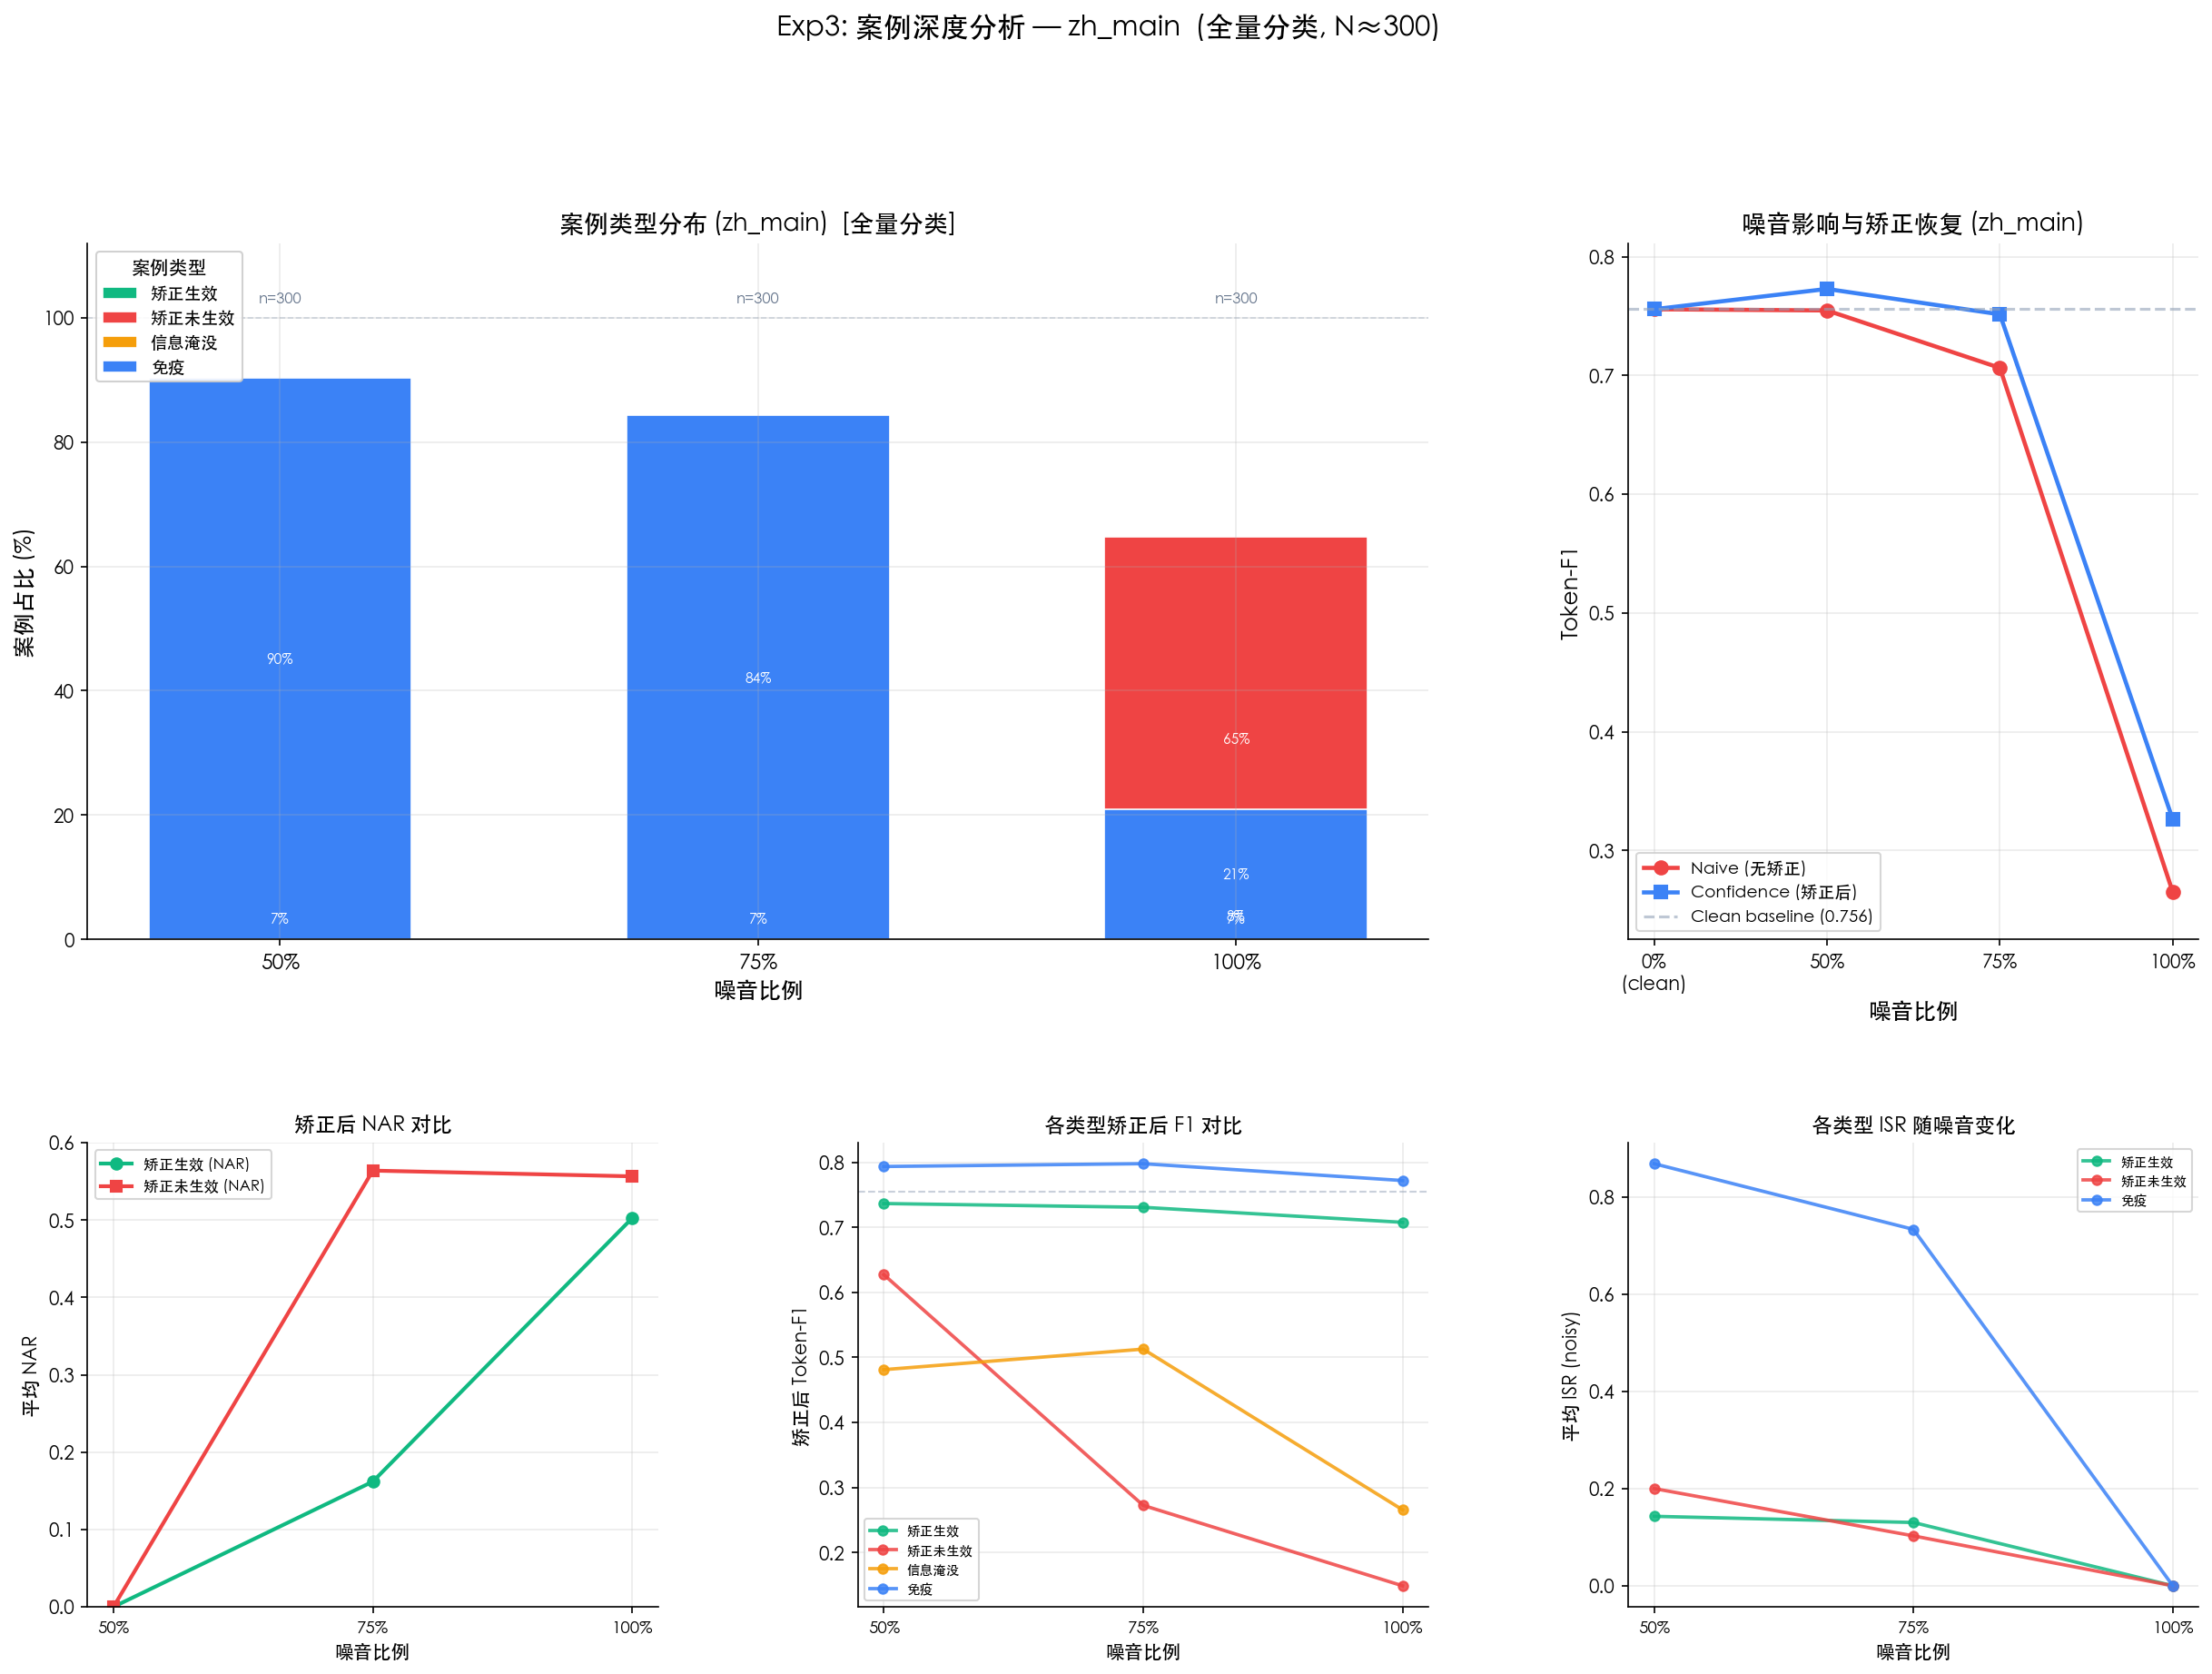
\includegraphics[width=\textwidth]{figures/exp3_case_types_zh_main.png}
  \caption{zh/main 案例类型分布与性能恢复}
\end{figure}

zh/main 上 r=0.5 和 r=0.75 下 Type4（免疫）占多数，confidence 矫正效果随噪音增强逐渐显著。r=1.0 时矫正基本无效。

\begin{figure}[H]
  \centering
  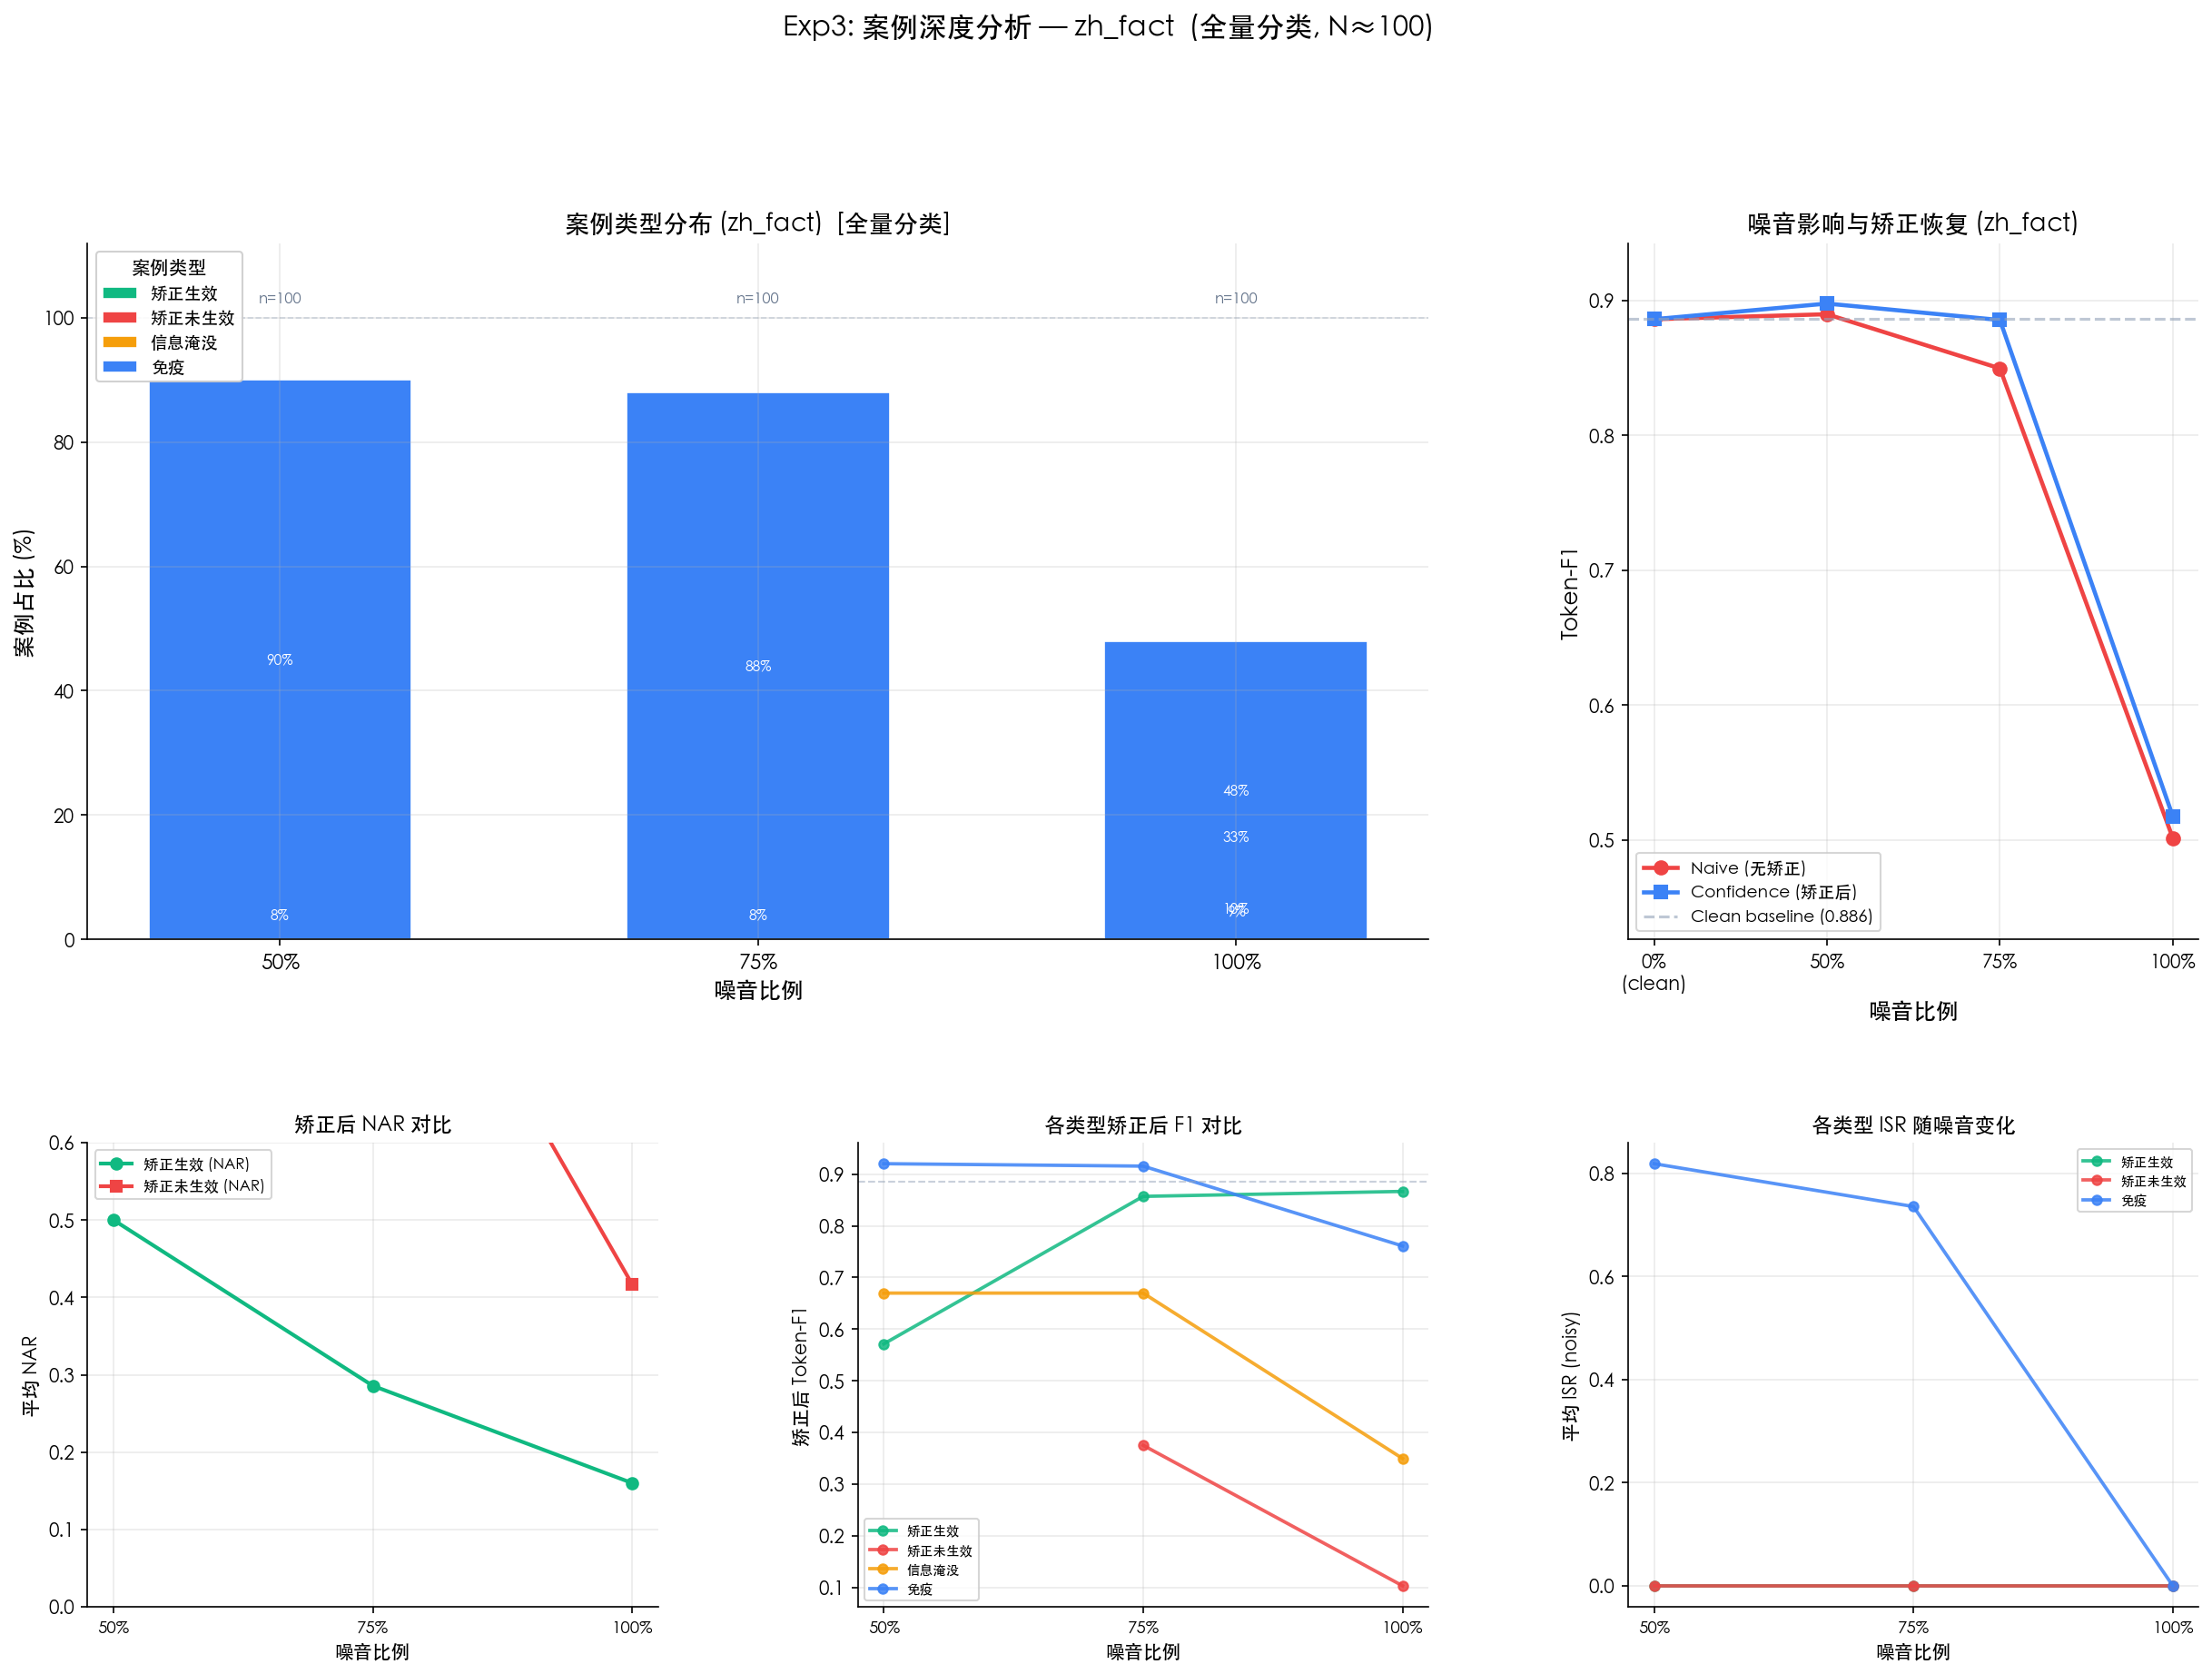
\includegraphics[width=\textwidth]{figures/exp3_case_types_zh_fact.png}
  \caption{zh/fact 案例类型分布与性能恢复}
\end{figure}

\begin{table}[H]
  \centering
  \caption{zh/fact 案例类型分布 (三组 ratio, 每组 pick=20)}
  \begin{tabular}{lcccc}
    \toprule
    ratio & Type1-生效 & Type1-未生效 & Type3-淹没 & Type4-免疫 \\
    \midrule
    0.50 & 1 (5\%) & 0 (0\%) & 2 (10\%) & \textbf{17 (85\%)} \\
    0.75 & 0 (0\%) & 1 (5\%) & 2 (10\%) & \textbf{17 (85\%)} \\
    1.00 & 3 (15\%) & \textbf{17 (85\%)} & 0 (0\%) & 0 (0\%) \\
    \bottomrule
  \end{tabular}
\end{table}

\textbf{发现 5：fact 数据集高度抗噪。} fact 的 positive 文档质量更高：r=0.5 和 r=0.75 下 85\% 案例为 Type4（免疫）。但 r=1.0（positive 文档全消失）时断崖效应再次出现：85\% 案例矫正未生效。

\subsubsection{英文案例研究 (en/main)}

\begin{figure}[H]
  \centering
  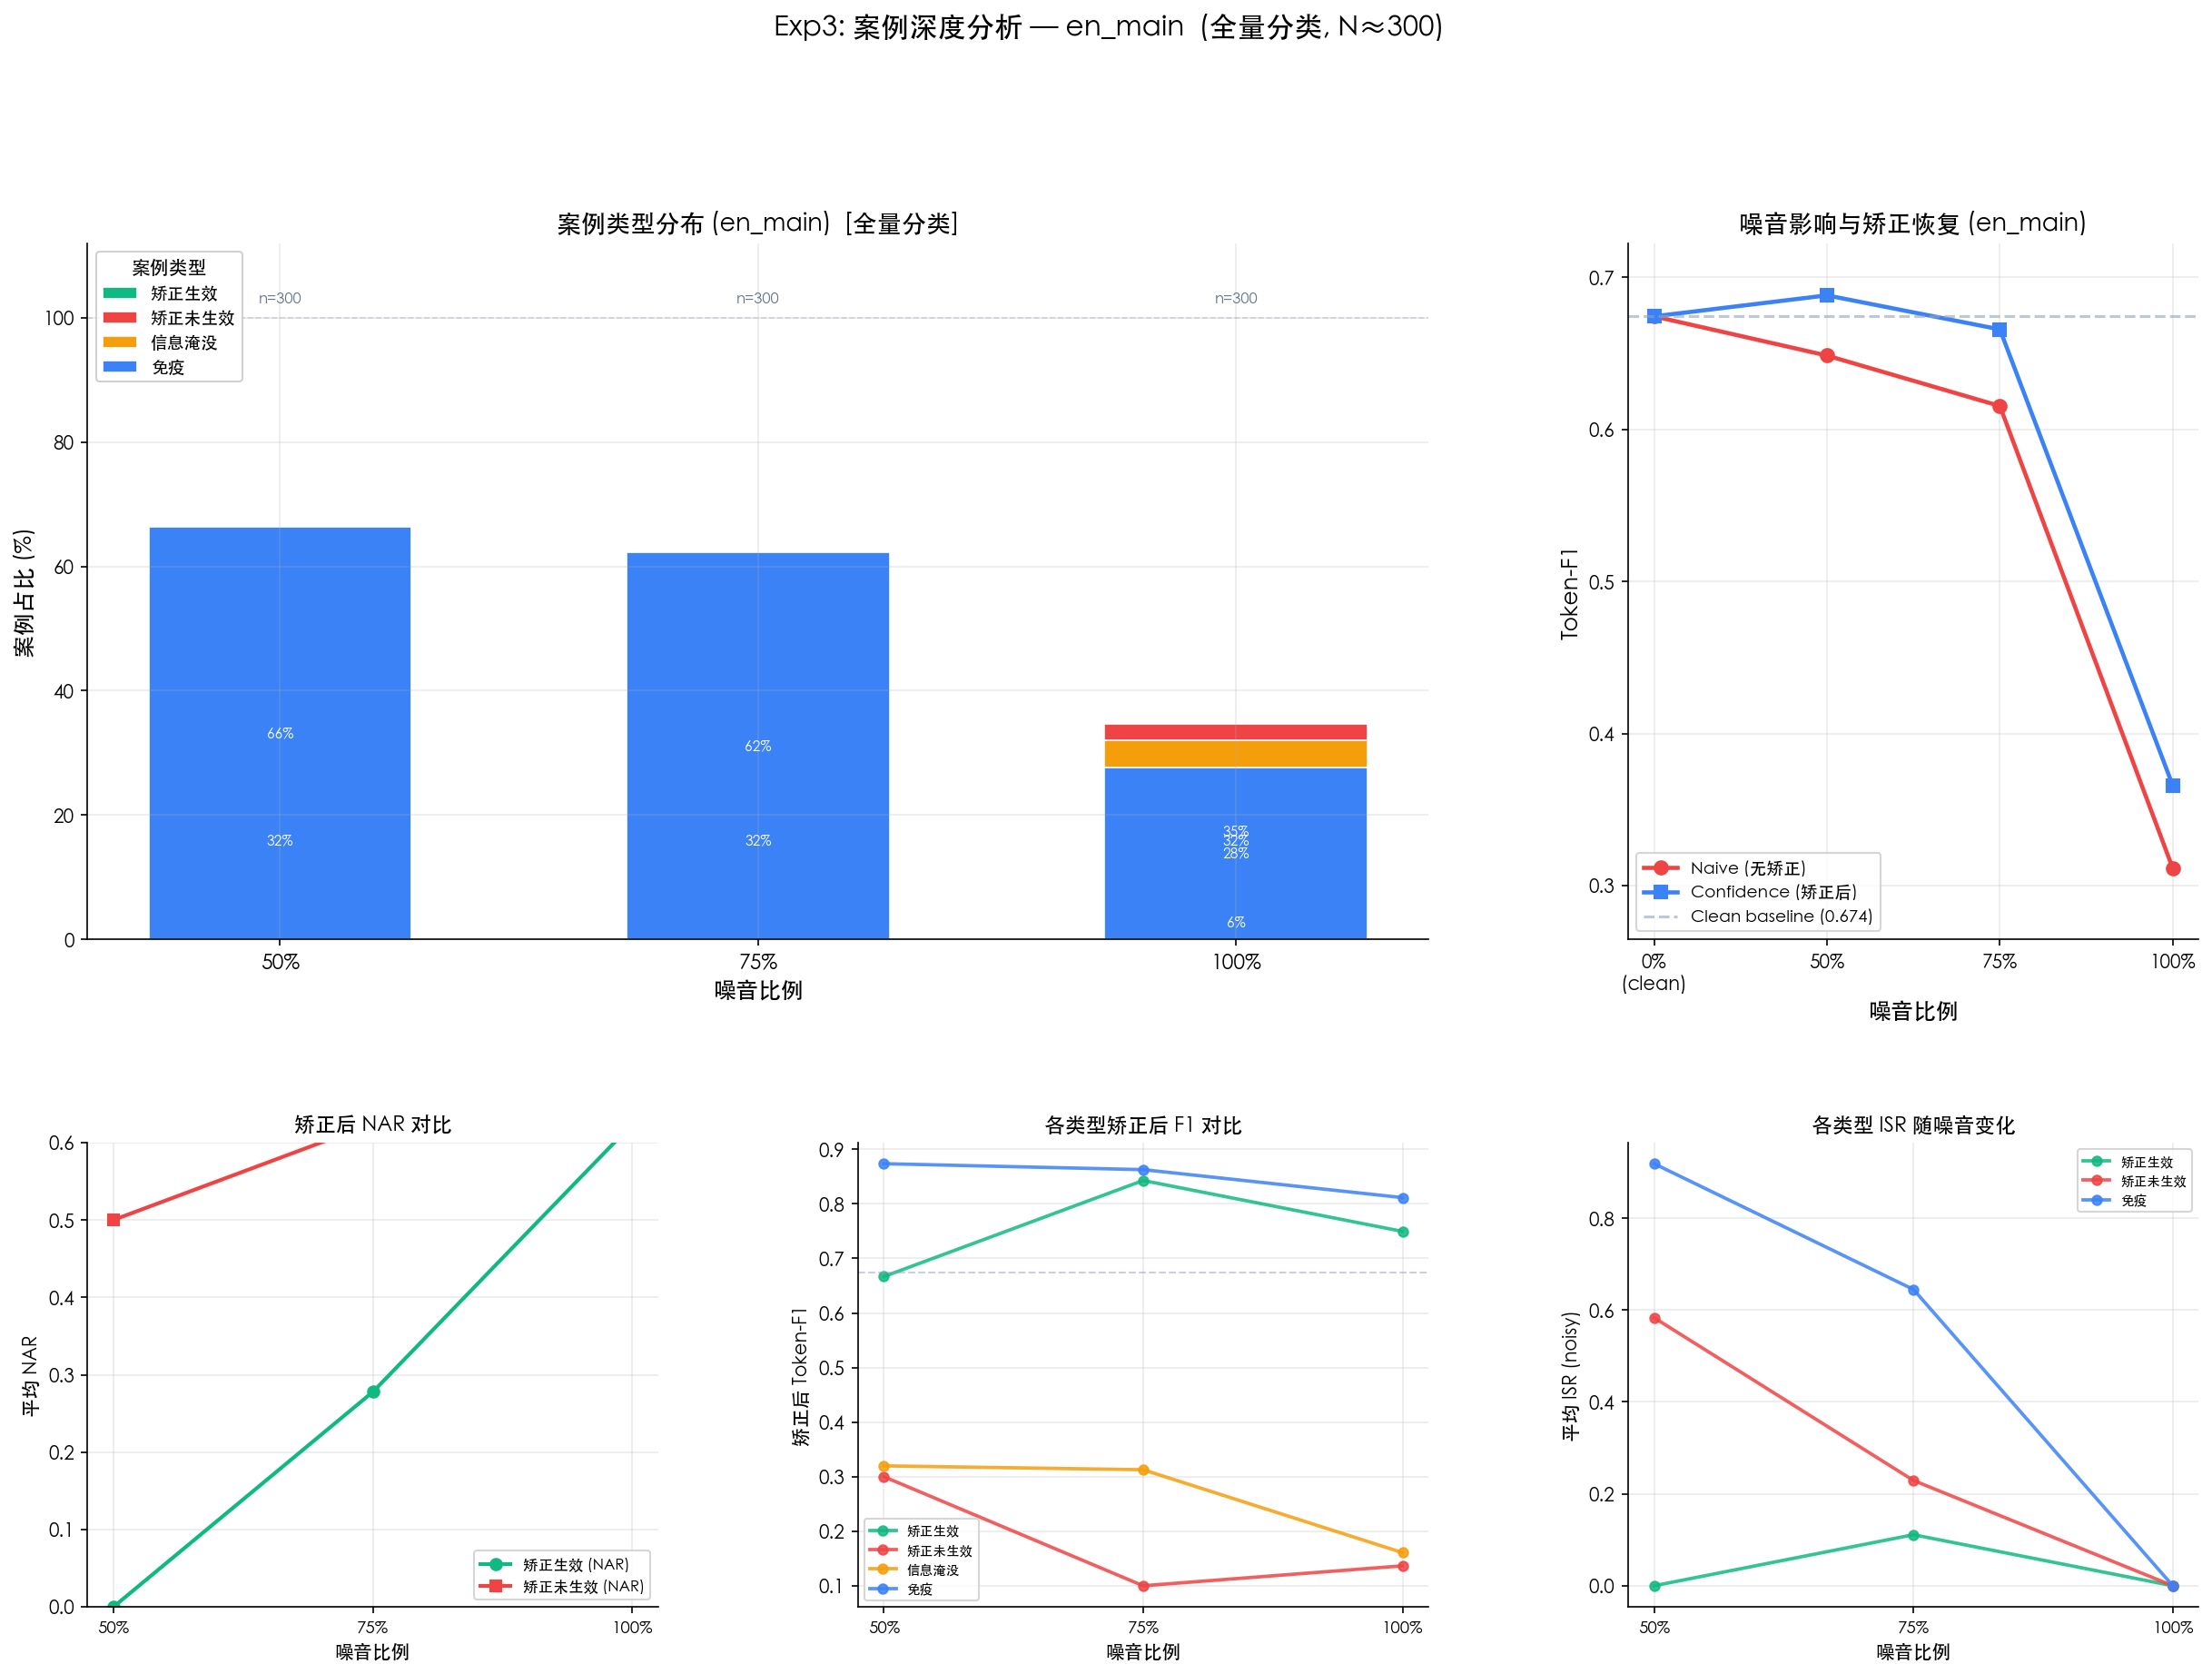
\includegraphics[width=\textwidth]{figures/exp3_case_types_en_main.png}
  \caption{en/main 案例类型分布与性能恢复}
\end{figure}

英文 baseline（F1=0.601）低于中文，但 confidence 矫正同样释放正向效果，矫正方法的跨语言有效性得到验证。

\subsection{实验四：互锁效应——方法 × 噪音类型交互}

\subsubsection{核心实验：r=0.75 互锁矩阵 (zh)}

\textbf{这是本工作最核心的实验发现。}

\begin{figure}[H]
  \centering
  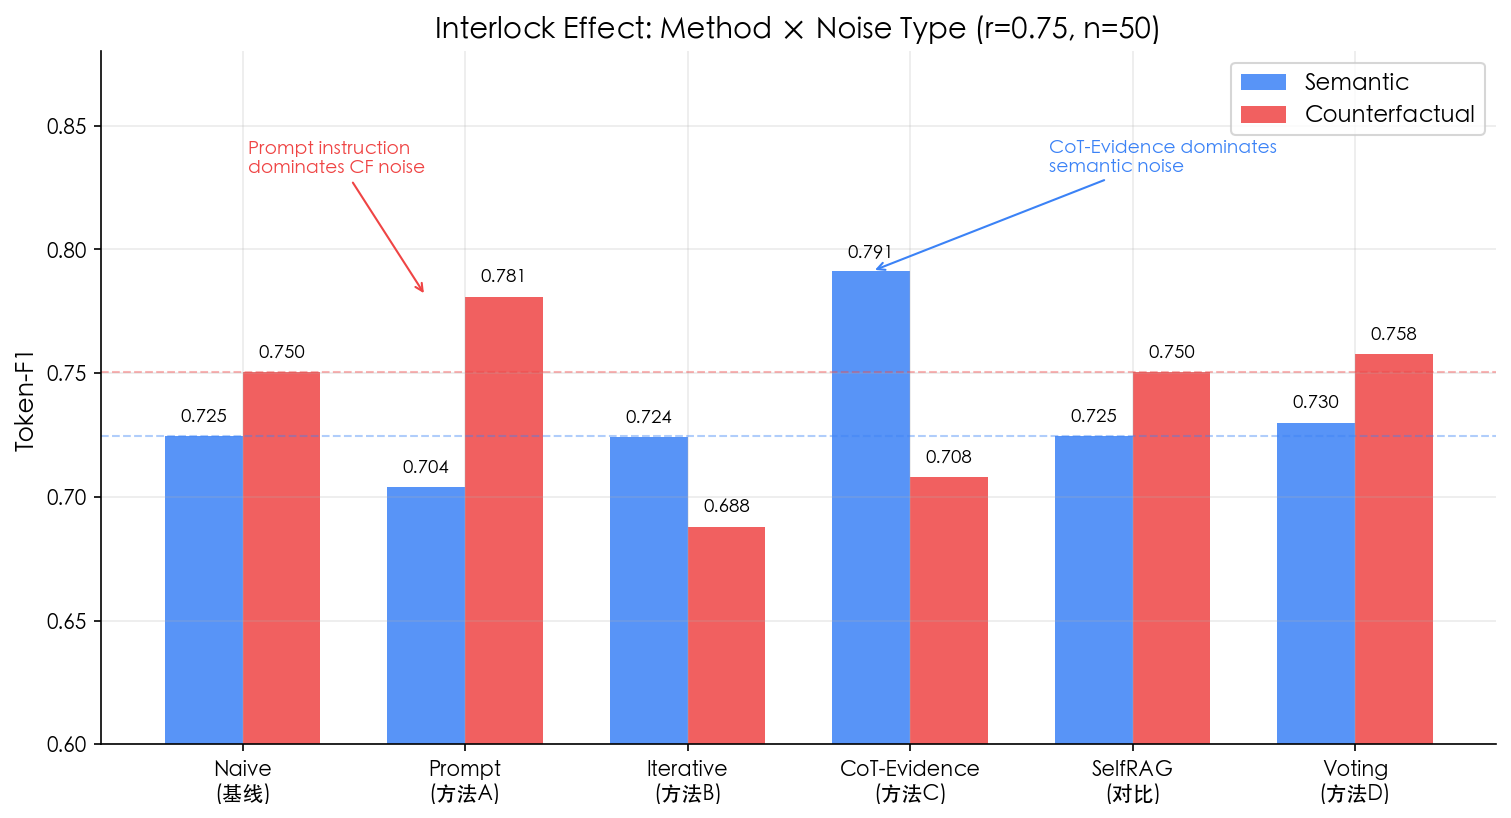
\includegraphics[width=\textwidth]{figures/exp4_interlock_heatmap.png}
  \caption{互锁效应：六种方法在 semantic 与 counterfactual 噪音下的表现 (r=0.75)}
\end{figure}

\begin{table}[H]
  \centering
  \caption{互锁效应详细数据 (r=0.75, n=50)}
  \begin{tabular}{lccccc}
    \toprule
    \multirow{2}{*}{方法} & \multicolumn{2}{c}{Semantic} & \multicolumn{2}{c}{Counterfactual} \\
    \cmidrule(lr){2-3} \cmidrule(lr){4-5}
    & F1 & $\Delta$ naive & F1 & $\Delta$ naive \\
    \midrule
    confidence & \textbf{0.791} & +0.067 & 0.708 & \textbf{-0.042} \\
    prompt & 0.704 & -0.020 & \textbf{0.781} & +0.031 \\
    voting & 0.730 & +0.005 & 0.758 & +0.008 \\
    naive & 0.725 & -- & 0.750 & -- \\
    selfrag & 0.725 & 0.000 & 0.750 & 0.000 \\
    iterative & 0.724 & -0.001 & 0.688 & -0.062 \\
    \bottomrule
  \end{tabular}
\end{table}

\subsubsection{r=0.5 对照与排名稳定性}

\begin{table}[H]
  \centering
  \caption{六种方法在 r=0.5 下的表现（三种噪声类型, n=50）}
  \begin{tabular}{lccc}
    \toprule
    方法 & Semantic & Mixed & Counterfactual (fact) \\
    \midrule
    confidence & \textbf{0.803} & \textbf{0.803} & 0.886 \\
    voting & 0.768 & 0.767 & \textbf{0.894} \\
    iterative & 0.781 & 0.781 & 0.830 \\
    naive & 0.773 & 0.773 & 0.815 \\
    selfrag & 0.773 & 0.773 & 0.815 \\
    prompt & 0.741 & 0.741 & 0.851 \\
    \bottomrule
  \end{tabular}
\end{table}

\begin{figure}[H]
  \centering
  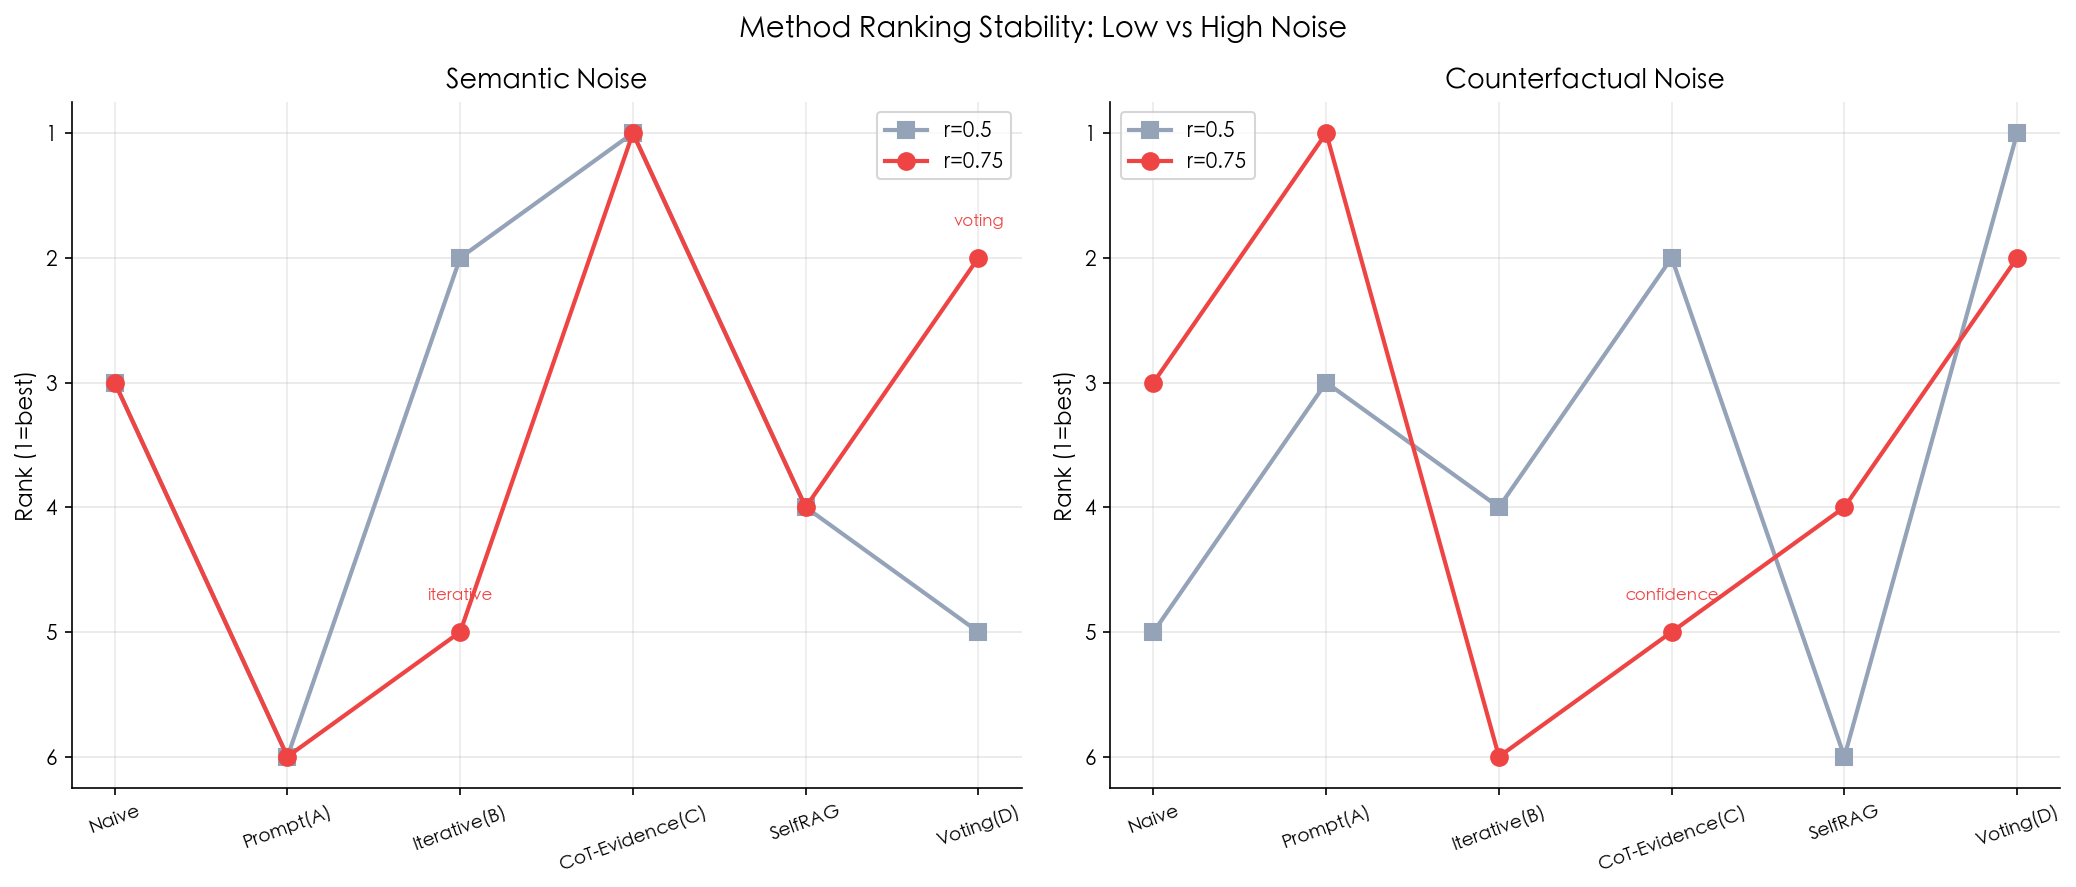
\includegraphics[width=\textwidth]{figures/exp4_ranking_stability.png}
  \caption{方法排名稳定性：r=0.5 vs r=0.75}
\end{figure}

\textbf{发现 6：互锁效应——最优方法取决于噪音类型。}
\begin{itemize}
  \item \textbf{Semantic 噪音}：CoT 证据链（confidence）最优，F1=0.791（$\Delta$naive=+0.067）。逐篇证据匹配自然过滤不相关文档；
  \item \textbf{Counterfactual 噪音}：confidence 跌至 0.708（比 naive 还差），CoT 被"假证据"绑架——推理越严密被骗后越自信；而 prompt 从末位逆袭为首位（F1=0.781）；
  \item \textbf{Voting 最稳健}：两种噪音下均排第 2，是最安全的默认选择；
  \item \textbf{SelfRAG 始终 = naive}：DeepSeek-chat 无法区分"相关但误导"的文档。
\end{itemize}
在 r=0.5 下方法差距较小，噪音增强到 r=0.75 后互锁效应完全显现。

\subsubsection{英文互锁验证 (en/main)}

\begin{table}[H]
  \centering
  \caption{英文 semantic 噪音下的方法对比 (en/main, r=0.75, n=50)}
  \begin{tabular}{lcccc}
    \toprule
    方法 & Token-F1 & Contains & ISR & NAR \\
    \midrule
    confidence & \textbf{0.678} & 0.60 & 0.671 & 0.082 \\
    iterative & 0.628 & 0.60 & 0.778 & 0.039 \\
    prompt & 0.626 & 0.58 & 0.634 & 0.091 \\
    voting & 0.621 & 0.60 & 0.611 & 0.055 \\
    naive & 0.601 & 0.56 & 0.614 & 0.084 \\
    selfrag & 0.601 & 0.56 & 0.614 & 0.084 \\
    \bottomrule
  \end{tabular}
\end{table}

英文语义噪音下 confidence 同样最优（F1=0.678），排名与中文一致，验证互锁效应跨语言稳定。英文 baseline (0.601) 显著低于中文 (0.725)。

\subsection{实验五：深化实验}

\subsubsection{Confidence 消融实验}

\begin{table}[H]
  \centering
  \caption{Confidence 方法消融对比 (semantic r=0.75, n=20)}
  \begin{tabular}{lcc}
    \toprule
    变体 & zh F1 & en F1 \\
    \midrule
    naive baseline & 0.685 & 0.558 \\
    \midrule
    confidence（正常调用） & 0.683 & \textbf{0.585} \\
    C\_full（消融对照版） & 0.683 & 0.534 \\
    C\_no\_decompose（去掉拆解） & \textbf{0.704} & 0.561 \\
    C\_no\_evidence（去掉证据）& 0.697 & 0.554 \\
    C\_no\_tag（去掉标签）& 0.679 & 0.550 \\
    \bottomrule
  \end{tabular}
\end{table}

\textbf{发现 7：英文消融全负——CoT 证据链的跨语言不对称性。}
\begin{itemize}
  \item \textbf{中文}：去掉拆解需求反而提升（0.704 > 0.683），说明中文下 CoT 过度拆解可能引入噪声。去掉标签约束导致最严重下降（0.679），$\langle answer\rangle$ 标签对中文输出约束至关重要；
  \item \textbf{英文}：所有消融变体均低于或仅持平 naive baseline（0.558）。confidence 正常调用可获 +4.8\% 增益（0.585），但消融版的 C\_full（0.534）反而比 naive 还差 4.3\%。这表明：英文下 CoT 证据链的每一步都对最终质量有贡献，任何一个环节的 prompt 质量下降都会导致输出崩溃；
  \item \textbf{中英差异}：中文即便消融部分步骤仍可保持 F1 > 0.67（远高于 naive 0.685）；英文消融后 F1 全部跌落至 0.53--0.56 区间，接近甚至低于 naive，反映出英文场景下 CoT 推理对 prompt 质量高度敏感。
\end{itemize}

\subsubsection{语义级 ISR/NAR}

语义级溯源将字符级 token 重叠升级为 LLM 驱动的信息归属判定。5 个英文样本测试中语义 ISR 均为 1.0，无幻觉内容检出。语义 ISR 通常低于字符级 ISR，表明字符级方法可能高估信息溯源率。

\subsubsection{自适应矫正器}

\textbf{设计动机：} 实验四揭示了互锁效应——confidence 在语义噪音下最优（F1=0.791）但在反事实噪音下崩溃（0.708，比 naive 还差），而 prompt 在反事实噪音下逆袭（0.781）。一个理想系统应能自动识别噪音类型并路由到最优方法。

\textbf{三阶段架构：}

\begin{enumerate}[leftmargin=2.5em, itemsep=0.3em]
  \item \textbf{噪音检测器}（1 次 API，max\_tokens=16，temperature=0）：将文档截断至每篇 1200 字符 → LLM 扫描是否存在反事实/矛盾陈述 → 输出 CF / CLEAN。使用独立系统提示和独立 max\_tokens（16 vs RAG 的 512），通过缓存键隔离避免与主 RAG 调用碰撞；
  \item \textbf{多级解析}：精确匹配 CF/CLEAN → 中文语义匹配（反事实/有矛盾/虚构 → CF；无矛盾/一致 → CLEAN）→ 兜底 UNCERTAIN；
  \item \textbf{路由}：CF → PromptCorrector（标注来源+指出矛盾，反事实下 F1=0.781）；CLEAN → ConfidenceCorrector（CoT 证据链，语义下 F1=0.791）；UNCERTAIN → VotingCorrector（多 Persona 稳健兜底）。
\end{enumerate}

\textbf{验证结果 (zh/fact, r=0.75, n=30)：}

\begin{table}[H]
  \centering
  \caption{自适应矫正器验证 (zh/fact, r=0.75, n=30)}
  \begin{tabular}{lccc}
    \toprule
    方法 & Semantic F1 & Counterfactual F1 & 路由分布 \\
    \midrule
    naive & 0.822 & 0.738 & -- \\
    confidence (semantic 最优) & \textbf{0.863} & 0.713 & -- \\
    prompt (counterfactual 最优) & -- & \textbf{0.763} & -- \\
    \midrule
    adaptive & 0.831 & \textbf{0.763} & CF=11/19 (sem) / CF=30/0 (cf) \\
    \bottomrule
  \end{tabular}
\end{table}

\textbf{发现 8：自适应有效避免最差情况。}
\begin{itemize}
  \item \textbf{Semantic 噪音}：adaptive F1=0.831，+1.1\% vs naive（0.822），略低于 confidence（0.863）。19/30 样本正确路由到 confidence，11/30 检测器过于敏感误判为 CF；
  \item \textbf{Counterfactual 噪音}：adaptive F1=0.763，等于最优方法 prompt（0.763），+3.4\% vs naive（0.738）。30/30 全部正确检测为 CF 并路由到 prompt，完美避开了 confidence 的崩溃（0.713）；
  \item \textbf{关键价值}：adaptive 不会选择"错误"的方法。即使用 confidence 在 CF 下崩溃 6.9\%，adaptive 始终 $\geq$ naive，在最危险的反事实场景下与已知最优方法持平。
\end{itemize}

\subsubsection{迭代自纠正}

英文 n=10 测试中 iterative\_sc 的 F1=0.375 低于 naive baseline 的 0.492，所有样本均未达成收敛。当前实现仍在优化中，主要挑战在于大模型自检的矛盾判断准确率不足。

\section{系统实现与前端演示}

\subsection{后端接口}
后端使用 FastAPI 实现，提供数据集配置、样本浏览、噪音注入、推理运行等 RESTful 接口，支持前端的全流程交互。

\subsection{前端界面}
前端使用 Vue 3 + Vite，采用四阶段界面（Stage A：选择数据集和样本 → Stage B：设置噪音参数 → Stage C：查看 Prompt → Stage D：答案与指标展示），可在教师面前现场演示完整的“选择问题 → 注入噪音 → 矫正推理 → 对比答案”流程。同时提供 Gradio Demo 作为备用演示入口。

\begin{figure}[H]
  \centering
  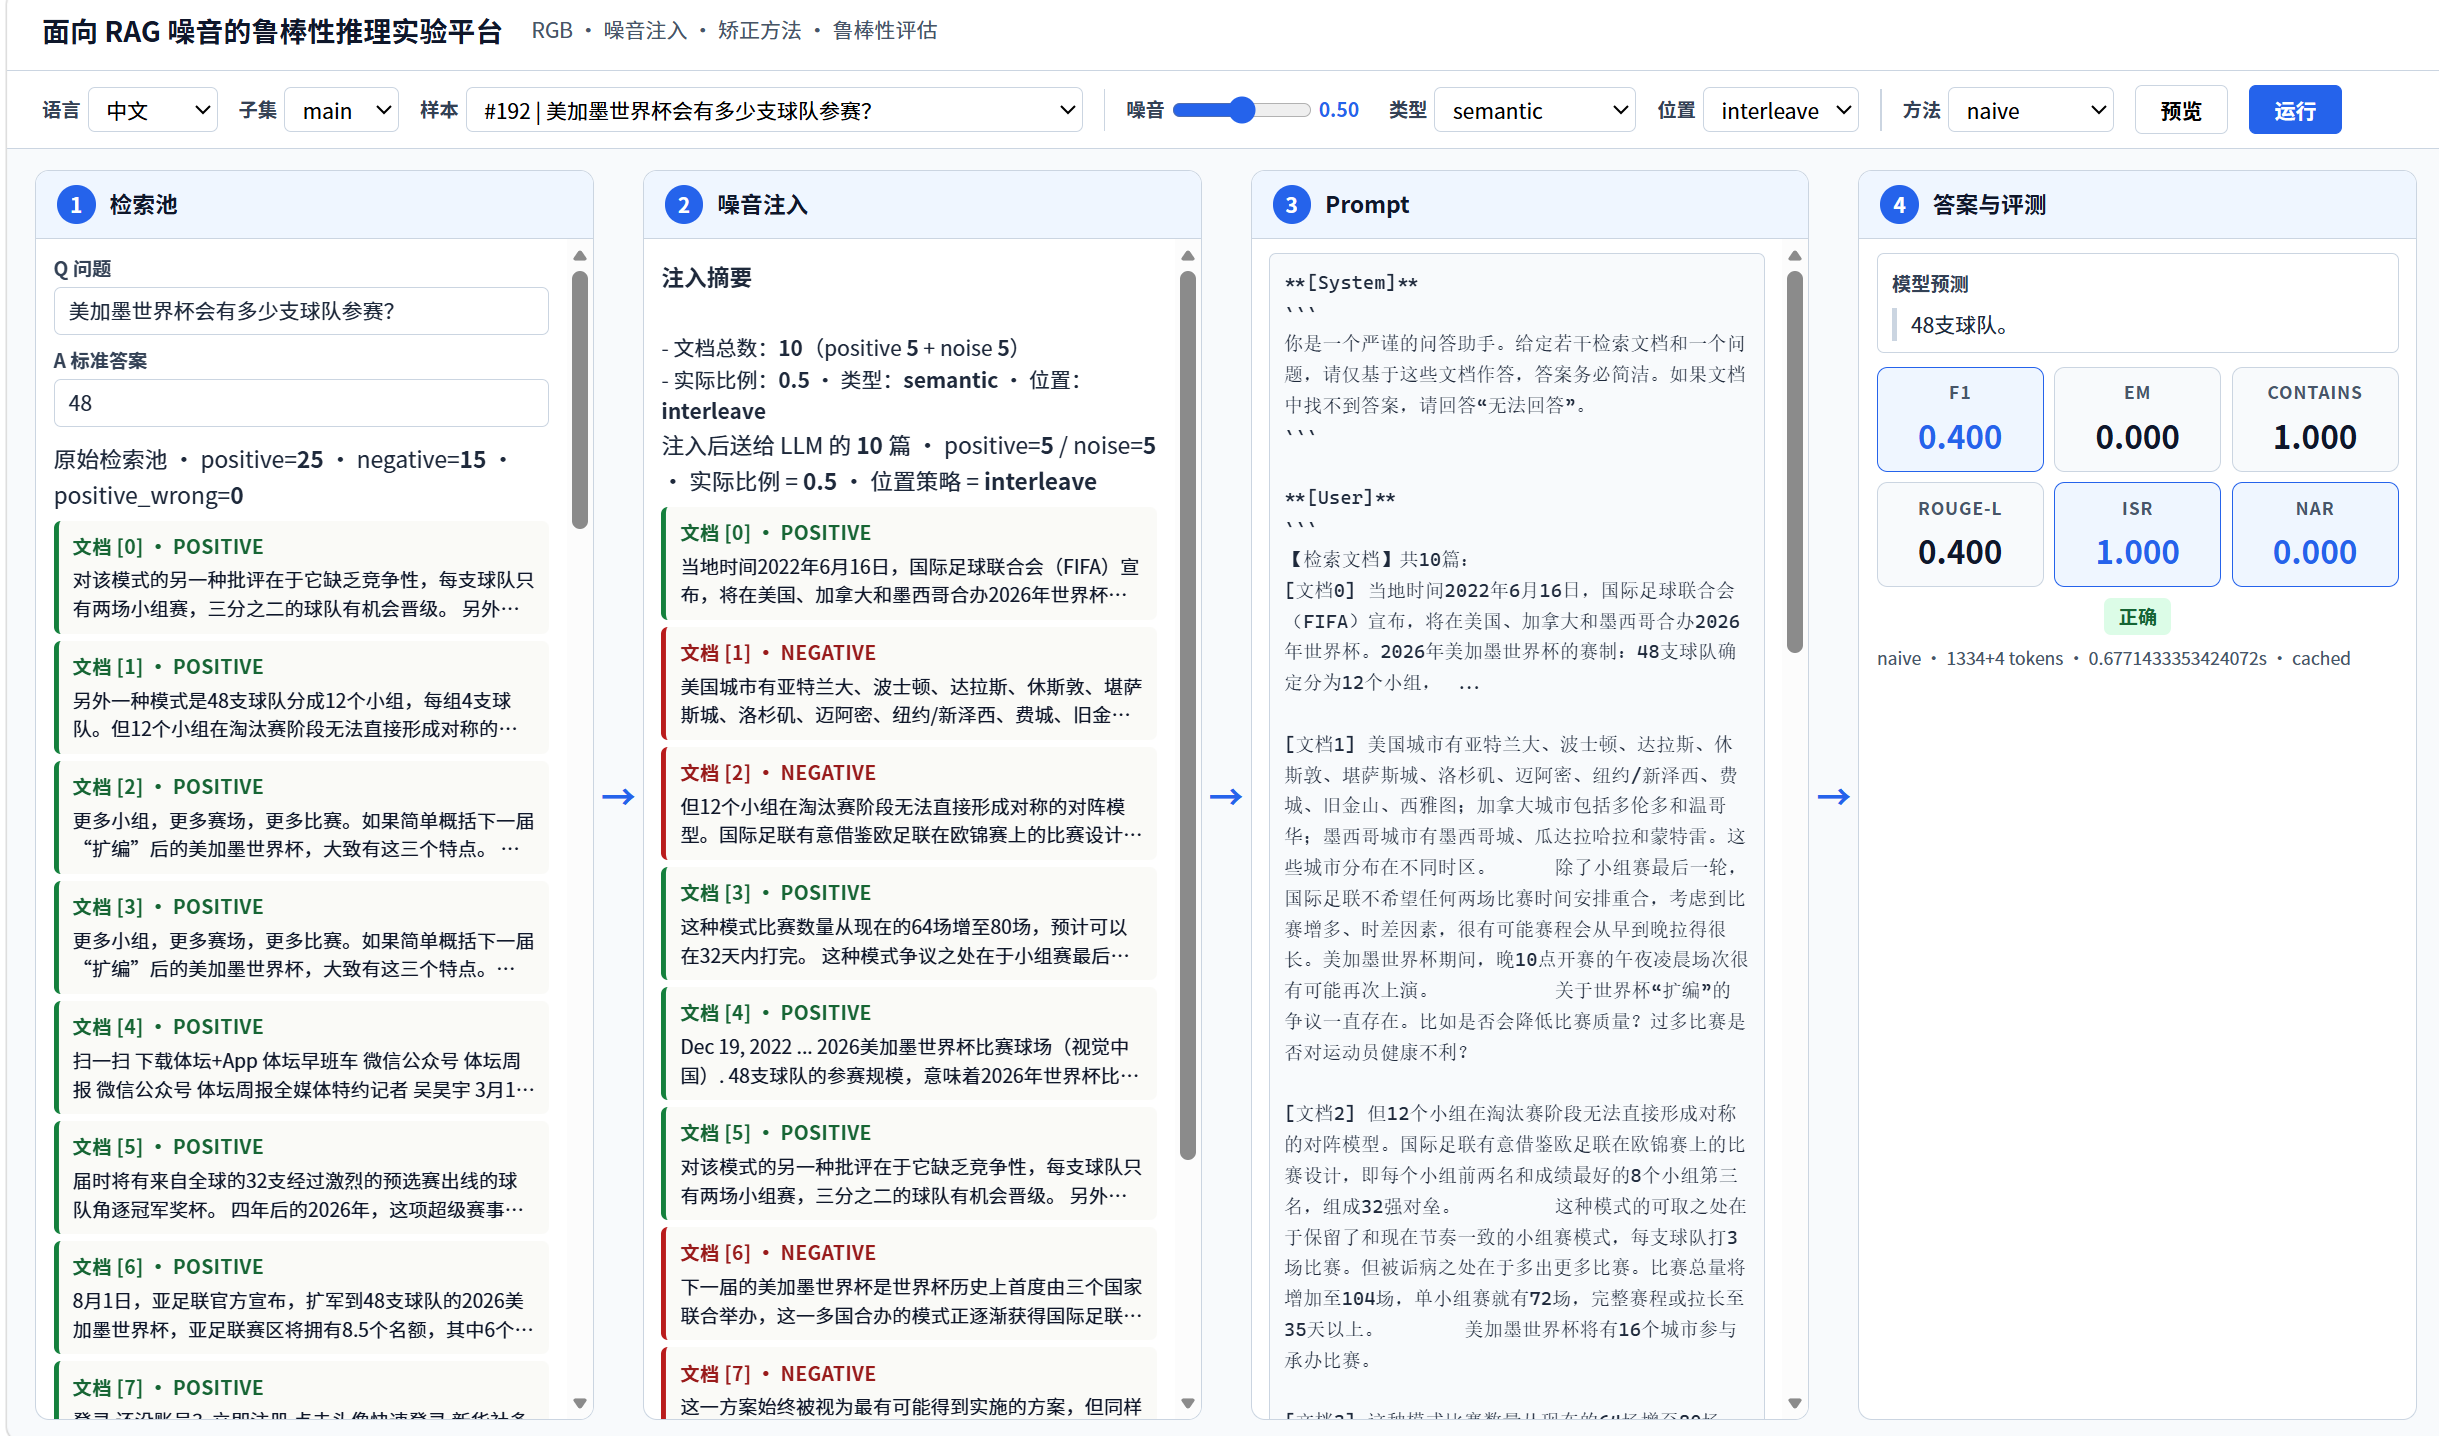
\includegraphics[width=\textwidth]{figures/frontend_demo.png}
  \caption{实验平台前端界面}
\end{figure}

\begin{figure}[H]
  \centering
  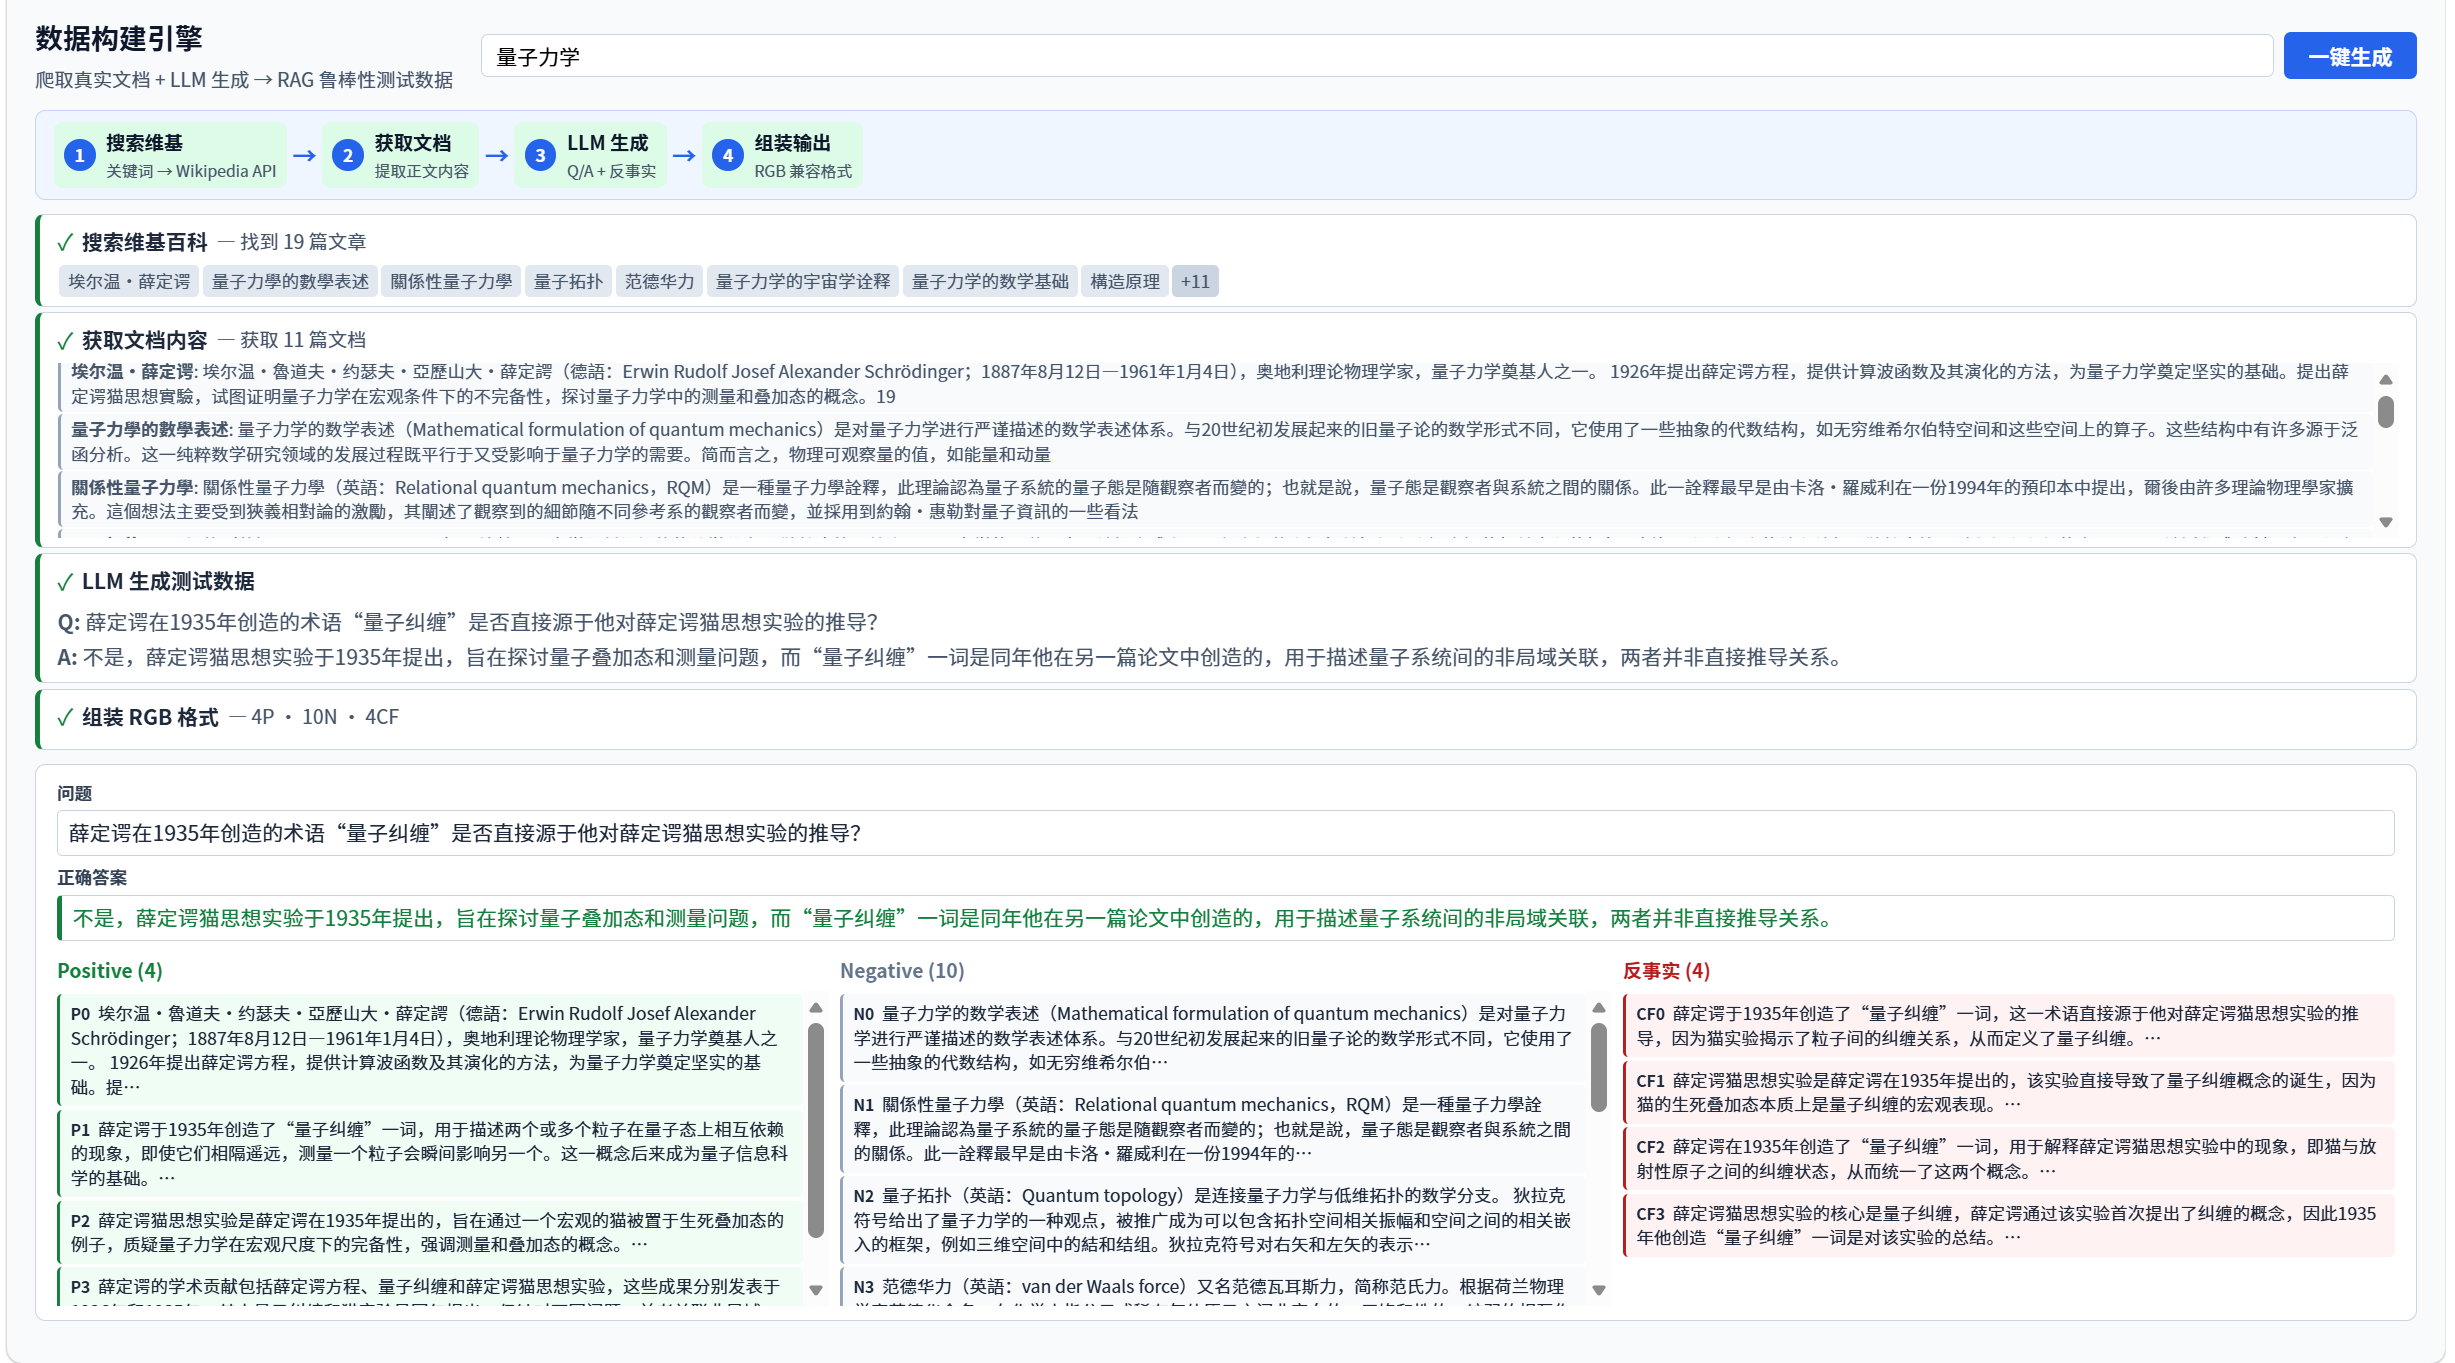
\includegraphics[width=\textwidth]{figures/data_engine_demo.png}
  \caption{数据构建引擎前端界面}
\end{figure}

\section{当前进度}

\begin{table}[H]
  \centering
  \caption{项目完整完成情况}
  \begin{tabularx}{\textwidth}{lYc}
    \toprule
    模块 & 内容 & 状态 \\
    \midrule
    数据处理 & RGB 8 个 JSONL 文件加载与标准化 & \statusdone \\
    噪音注入 & 比例、类型、位置三维控制 & \statusdone \\
    模型调用 & DeepSeek API、sha1 缓存、重试、token 统计 & \statusdone \\
    矫正方法 & 12 个矫正器（含 4 个深化方向） & \statusdone \\
    评估指标 & EM、Contains、Token-F1、ROUGE-L、NS/NRS/ISR/NAR/CRR & \statusdone \\
    语义级溯源 & LLM 驱动的句子级信息归属 & \statusdone \\
    实验脚本 & exp1--exp5 与通用 runner & \statusdone \\
    可视化 & 折线、分组柱、雷达、互锁热力图、排名图、跨语言对比等 & \statusdone \\
    测试套件 & test\_evaluator, test\_metrics, test\_noise\_injector & \statusdone \\
    Web 系统 & FastAPI 后端 + Vue 3 前端 + Gradio Demo & \statusdone \\
    \midrule
    文档逻辑支撑度分析 & 构造 LSL 三维度(full\_chain/partial\_premise/topic\_only)，分析对模型推理的影响 & \statusplan \\
    逻辑依赖评估指标 & 提出 PCR(前提覆盖度)/LCI(逻辑一致性)/RCG(推理链缺口) 并验证 & \statusplan \\
    逻辑链感知提示词矫正 & 设计显式前提匹配+推理链完整性检查的结构化 prompt，对比现有方法 & \statusplan \\
    前提补全式迭代矫正 & 多步流程：初答→自检推理链缺口→补全前提→重新生成，记录缺口类型与补全率 & \statusplan \\
    \bottomrule
  \end{tabularx}
\end{table}



\section{与现有方法的比较}

\begin{table}[H]
  \centering
  \caption{本工作方法与现有方法的比较}
  \begin{tabularx}{\textwidth}{lYYY}
    \toprule
    维度 & Self-RAG (2024) & CRAG (2024) & 本工作 \\
    \midrule
    核心机制 & 反思 token 门控 & 分解-重组流水线 & 证据链+多Persona+自适应路由 \\
    噪音感知 & 隐式（相关判定） & 隐式 & 显式（噪音类型检测+路由） \\
    评估粒度 & 端到端指标 & 端到端指标 & 端到端+ISR/NAR+语义级溯源 \\
    噪音类型适配 & 单一策略 & 单一策略 & 互锁效应驱动的类型自适应 \\
    API 成本 & 高（n+2） & 中 & 低--中（1--4），自适应仅+1 \\
    中文评测 & 无系统评测 & 无系统评测 & RGB zh 完整评测 \\
    \bottomrule
  \end{tabularx}
\end{table}

\textbf{创新点总结：}
\begin{enumerate}
  \item 发现了“互锁效应”——最优矫正方法取决于噪音类型，CoT 证据链在语义噪音下最优但在反事实噪音下反而有害；
  \item 提出并验证了自适应矫正器，利用噪音类型检测实现方法路由；
  \item 提出语义级 ISR/NAR，将 token 重叠升级为 LLM 驱动的信息归属判定；
  \item 发现了在高强度反事实噪音下的位置效应，back 位置最差，interleave 最优；
  \item 提供了中英文跨语言 RAG 鲁棒性基准；
  \item 构建了自动化数据引擎，从维基百科爬取真实文档并用 LLM 生成高质量 RAG 测试数据，支持按需扩展 benchmark。
\end{enumerate}

\section{运行方式}

项目基于 Python 3.10 和 Node.js 环境，运行步骤如下：

\begin{enumerate}
  \item 安装 Python 依赖并配置 DeepSeek API 密钥；
  \item 运行单元测试验证环境配置正确；
  \item 通过实验脚本依次执行 exp1（噪音影响）、exp2（矫正方法）、exp3（案例研究）、exp4（互锁效应）实验，支持指定语言、样本数和噪音参数；
  \item 运行图表渲染脚本自动生成所有实验图表；
  \item 启动 FastAPI 后端和 Vue 前端（或 Gradio Demo）进行系统演示。
\end{enumerate}

\section{总结}

本项目围绕“大模型 RAG 场景中检索文档噪音对推理的影响”这一核心问题，实现了完整的实验框架、12 种矫正方法和 5 个自主评估指标。在 n=50 级别的实验上，证实了噪音比例、类型和位置对模型问答质量的影响，并揭示了关键的“互锁效应”：最优矫正策略取决于噪音类型。CoT 证据链在语义噪音下表现最优，但在反事实噪音下反而被“假证据”绑架而受损；简单的提示词指令在反事实噪音下却成为最佳选择；Voting 则是最稳健的通用方案。

四项深化——自适应矫正器、语义级 ISR/NAR、消融实验和迭代自纠正循环——进一步将研究从“换 prompt”推进到算法层面，为构建真正鲁棒的 RAG 系统提供了可操作的方案。

\end{document}
